\chapter{Evaluation}
\label{cpt:evaluation}

As Chakroborty argued, any part of railway signaling requires highly reliable and fault-tolerant design~\cite{ChakrabortyFaultTolerantRailway}.
Various methods exist to achieve these requirements from which redundancies and recovery mechanisms were used.
Chakroborty further states that redundancy can only support reliability and safety when it is managed correctly.
Therefore, the developed system is analyzed and assessed to evaluate the applied redundancies' correctness.
\\

In the first section of this chapter, a program - called \textit{simulator} - for simulating train movement and journeys is presented.
Based on the simulated journeys, the developed system can be automatically tested in different situations.
In the second section, the system's functionality, reliability, and safety are evaluated regarding four criteria.
First, the applied network's data transmission is analyzed.
Second, the on-board system's resource utilization is measured and assessed.
Third, leader election times are measured to analyze the worst-case time that the system can be without a leader.
Fourth, the simulator is used to evaluate how the system supervises the train's movement and processes input messages, even if individual components fail.
Finally in this chapter, a \abr{DDS} subset for achieving the described behavior as well as advantages and challenges of applying \abr{DCPS} middleware in safety-critical systems are presented.


\section{Scenario Simulation}
\label{subsec:ScenarioSimulation}

\begin{figure}[!htb]
	\centering
	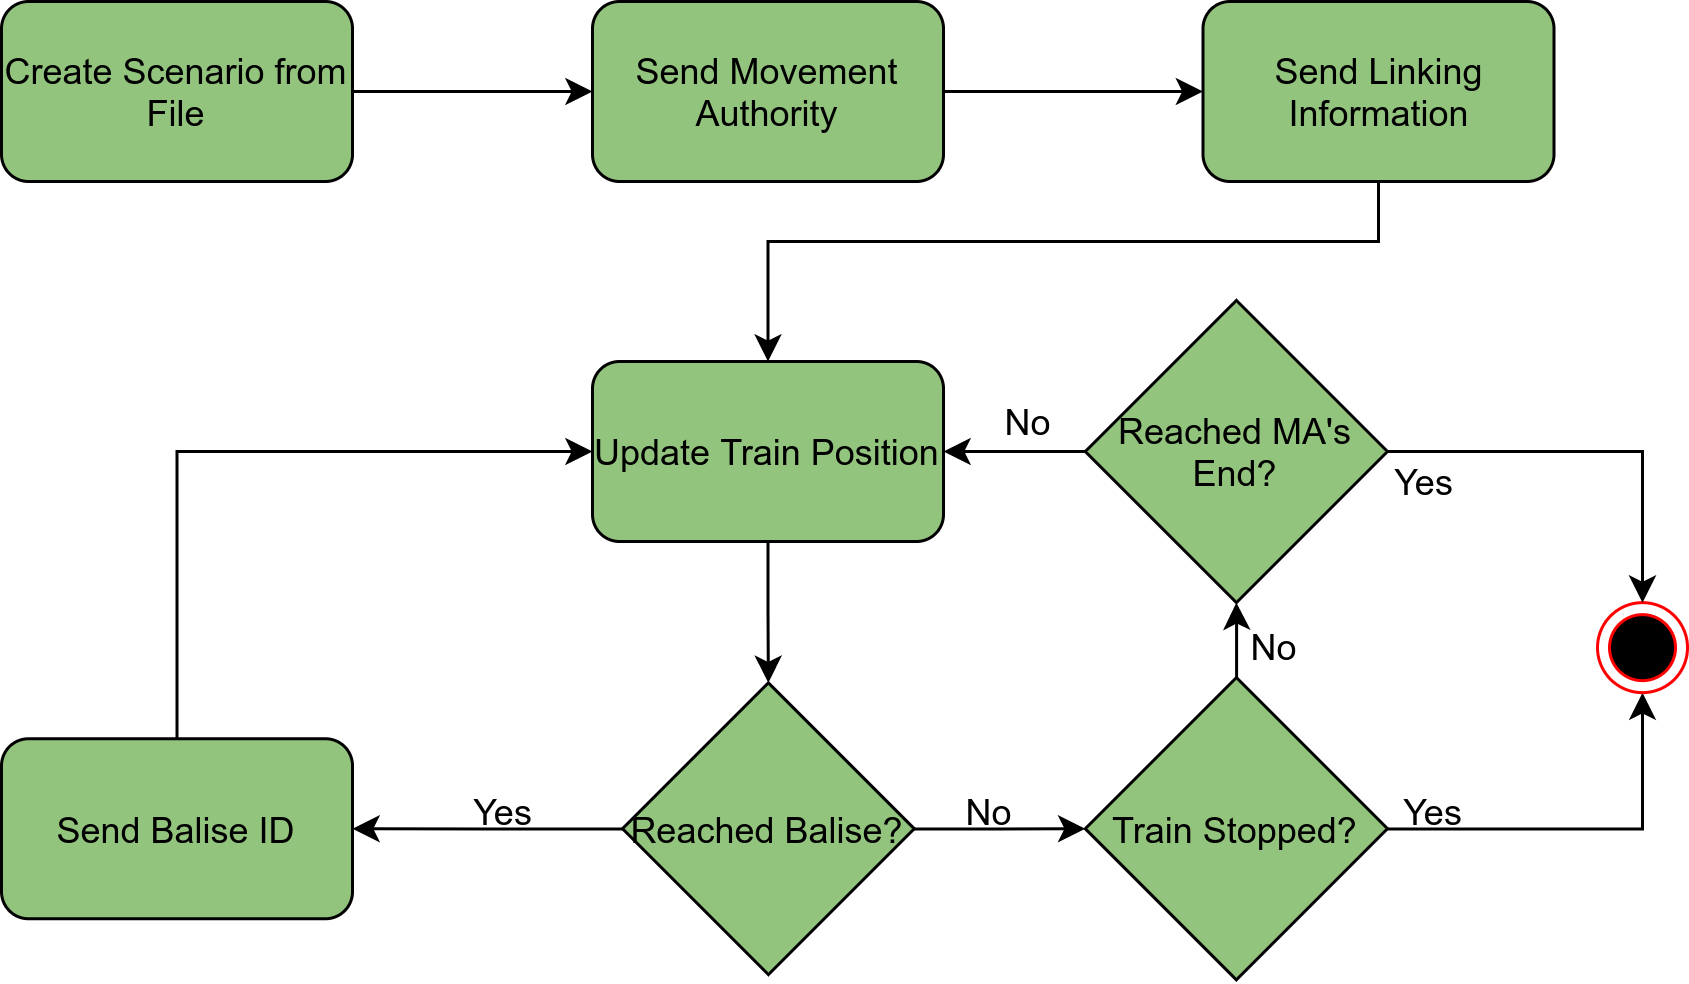
\includegraphics[width=0.8\linewidth]{images/SimulatorWorkflow}
	\caption{The workflow of a scenario simulation. Each simulation begins by creating a scenario from a file and sending \glsentryfull{MA} and linking information. Thereupon, the virtual train is set in motion and balise telegrams are send on its way. When the virtual train stops early or when the \abr{MA}'s end is reached, the simulation stops.}
	\label{fig:SimulatorWorkflow}
\end{figure}

The developed on-board system supervises a train while it is on a journey.
Each journey is encapsulated within a scenario that is bounded by a \abr{MA} and consists of a set of linked balises and track-side balises.
Scenarios are simulated to test the system and evaluate it concerning various criteria.
Therefore, the elected leader simulates the train's position based on a constant speed and a hypothetical sensor inaccuracy.
A separated program, called \textit{simulator}, simulates \abr{RBC} and track-side balises.
At the beginning of each scenario, the simulator provides a \abr{MA} and a set of linked balises to the on-board system.
Further, the simulator sends balise telegrams when the simulated train reaches a virtual track-side balise.
The workflow of how the simulator executes a scenario is depicted in~\autoref{fig:SimulatorWorkflow}.
\\

In a first step, a new scenario is created from a \textit{json} file.
An exemplary scenario in \textit{json} format is shown in~\autoref{code:scenarioJSON}.
In the depicted case, three track-side balises are simulated at three different positions.
The first two balises are linked while the third is not.
A distinction is made between the balise's position and its linked position in order to simulate the case that a balise is not at the position with which it was linked.

\begin{minipage}{\linewidth}
\begin{lstlisting}[caption={The developed simulator simulates scenarios that are provided in \texttt{json} format. Each scenario consists of a \abr{MA} with a start and an end position, as well as a set of balises. Balises can either be linked or not and include an identification number, a linking position, and a position. The linking position is used to simulate a misplaced balise.}, label=code:scenarioJSON]
{
  "MA": {
    "start": 0,
    "end": 10
  },
  "balises": {

    "balise": {
      "id": 0,
      "link_pos": 1,
      "pos": 1,
      "linked": true
    },
    "balise": {
      "id": 1,
      "link_pos": 5,
      "pos": 5,
      "linked": true
    },
    "balise": {
      "id": 2,
      "pos": 7,
      "linked": false
    }

  }
}

\end{lstlisting}
\end{minipage}

\subsection{Simulator Classification}

In literature, simulators are distinguished based on their mode of operation.
They are categorized into simulators based on \abr{DE}-, and \abr{CT}~\cite{CoSimulationStateOfTheArt}.
In a \abr{DE}-based simulation, communication with the environment is characterized by events that are triggered at certain times.
For \abr{CT}-based simulations, the simulated state is expected to evolve continuously over time.
Based on these properties, it can be argued that the simulator that is utilized in this work is a combination of a \abr{DE}- and a \abr{CT}-based simulation system.
On the one hand, the train's movement is simulated in a way that is typical to \abr{CT}-based simulations because the train's position continuously evolves over time based on its speed.
On the other hand, the track-side balise telegram simulation borrows features from \abr{DE}-based simulators because it communicates via events.

\subsection{Test Automation}
\label{subsec:testautomation}

Because the scenarios are simulated, a reproducible test environment is created.
This enables automated integration testing and facilitates the measurement of system characteristics under comparable circumstances.
Further, data reproducibility allows to make changes to the system and to evaluate its performance compared to other versions.
With the help of the simulator, the system can be continuously tested under different conditions and in different situations without using or jeopardizing real railway components.
\\

\begin{table}[h!]
	\begin{center}
		\caption{In order to test the system's behavior in critical situations, three scenarios - called \textit{test scenarios} - are used. Each \textit{test scenario} includes a \abr{MA} and three balises but differs in the number and position of linked balises. In \texttt{Reach End of \abr{MA}}, all three balises are linked. In \texttt{Unlinked Balise}, only the first two balises are linked and the third is not. In \texttt{Balise not where expected}, all three balises are linked but the third's balises linked position differs from its actual position. As a consequence, the system's expected behavior for each scenario is different.}
		\label{tab:simulatedScenarios}
		\begin{tabularx}{\textwidth}{|X|X|}
			\hline
			\textbf{Name} & \textbf{Expected behavior}\\
			\hline \hline
			Reach End of \abr{MA} & All balise telegrams are evaluated correctly and the train stops at the \abr{MA}'s end. \\
			\hline
			Unlinked Balise & The train stops when the third and unlinked balise is encountered. \\
			\hline
			Balise not where expected & The actual position of the last balise does not correspond with its linked position. The train stops when this balise is encountered. \\
			\hline
		\end{tabularx}
	\end{center}
\end{table}


The functional fault model envisages three situations that must lead to the train being stopped under all circumstances (ref.~\autoref{subsec:faultModel}).
For ensuring that these situations are always handled correctly, they are simulated in scenarios, which are - together with their expected behavior - shown in~\autoref{tab:simulatedScenarios}.
These three scenarios are called \textit{test scenarios}.
In order to facilitate automatic integration testing, the \abr{EVC}'s system logic has been patched to write the system's decisions to input messages and braking curve observations into a file called \textit{evaluation file}.
For each decision, the train's current position, the decision of whether the train should brake or continue driving, the last encountered balise, and a reason are saved.
A \texttt{Python} script is used to automatically evaluate whether the \abr{EVC} corresponds to its expected behavior.
Therefore, the script invokes the simulator for each scenario and, after the train stopped, analyzes the \textit{evaluation file}.
In this manner, the system's actual behavior can automatically be compared to its expected behavior.
By injecting different faults, for example manually crashing a replica, it can be validated whether the system is still safe and reacts as expected.


\section{System Evaluation}

In this section, the system's functionality, reliability, and safety are evaluated based on various measurements regarding resource utilization and exchanged messages.
Measurements were made both in idle mode and while processing the test scenarios (ref.~\autoref{tab:simulatedScenarios}).
In idle mode, the train is at a standstill, no input messages need to be evaluated, and only heartbeat messages are exchanged.

\begin{table}[h!]
	\begin{center}
		\caption{Nine topics are used in the system that each manages different data in a certain data format. As a result, each message that belongs to a particular topic has a fixed size except the \texttt{Input} topic. The \texttt{Input} topic is used to transmit different types of data and therefore maps to an identification number and a sequence of data with a length \textbf{l}.}
		\label{tab:topicMessageSize}
		\begin{tabularx}{\textwidth}{|X|X|}
			\hline
			\textbf{Topic} & \textbf{Message Size in Bytes} \\
			\hline \hline
			AppendEntries & 12 \\
			\hline
			AppendEntriesReply & 18 \\
			\hline
			RequestVote & 8 \\
			\hline
			RequestVoteReply & 13 \\
			\hline
			Input & $4 + 4 * l$  \\
			\hline
			ActivateSpare & 5 \\
			\hline
			LinkedBalises & 6 \\
			\hline
			TrainState & 41 \\
			\hline
			MovementAuthority & 8 \\
			\hline
		\end{tabularx}
	\end{center}
\end{table}

Components in the distributed system synchronize each other by exchanging messages via \abr{DDS} topics.
Each topic has a characteristic data structure that determines the message's content and size.
The size for each message sent via a given topic is listed in~\autoref{tab:topicMessageSize}.
\\

First in this section, the applied network's data transmission times and latencies are analyzed before its resource utilization is assessed.
Afterward, the consensus algorithm's leader election time is measured to analyze the worst-case time that the system can be without a leader.
Finally, the test scenarios are run one after the other.
The system's components thereby exchange messages that are captured, stored, and analyzed to reproduce the system's behavior in the process.

\subsection{Data Transmission}

An essential parameter for assessing a distributed system is network latency~\cite{SinhaMeasureNetworkLatency}.
Network latency is used to indicate a delay that occurs while data is transmitted via a network.

It can be derived from the network's throughput characteristic.
\\

In the analyzed architecture, components are arranged in a star topology and interconnected via a network switch that allows up to 2000 Mbit/s for each port.
Data is transmitted via a wired \textit{Ethernet} connection.
The interface of the utilized \textit{Revolution Pi} is a 10/100 Ethernet.
Consequently, data transfers with up to 100~MBit/s are theoretically possible.
In order to examine the bandwidth and latency of the applied network, a \abr{DDS} throughput testing program from \texttt{ADLINK} is used.
Further, a publisher has been set up on one replica and a receiver on another.
The publisher starts sending messages with different payload sizes and the subscriber counts the number of received bytes and samples.
The communication is state-based, i.e. \texttt{WaitSets} are used so that the test setup is comparable to the actual application.
Because the network has the same diameter between every node, the number of transferred bytes and samples is independent of publisher and subscriber placement.

\begin{figure}[!hbt]
	\centering
	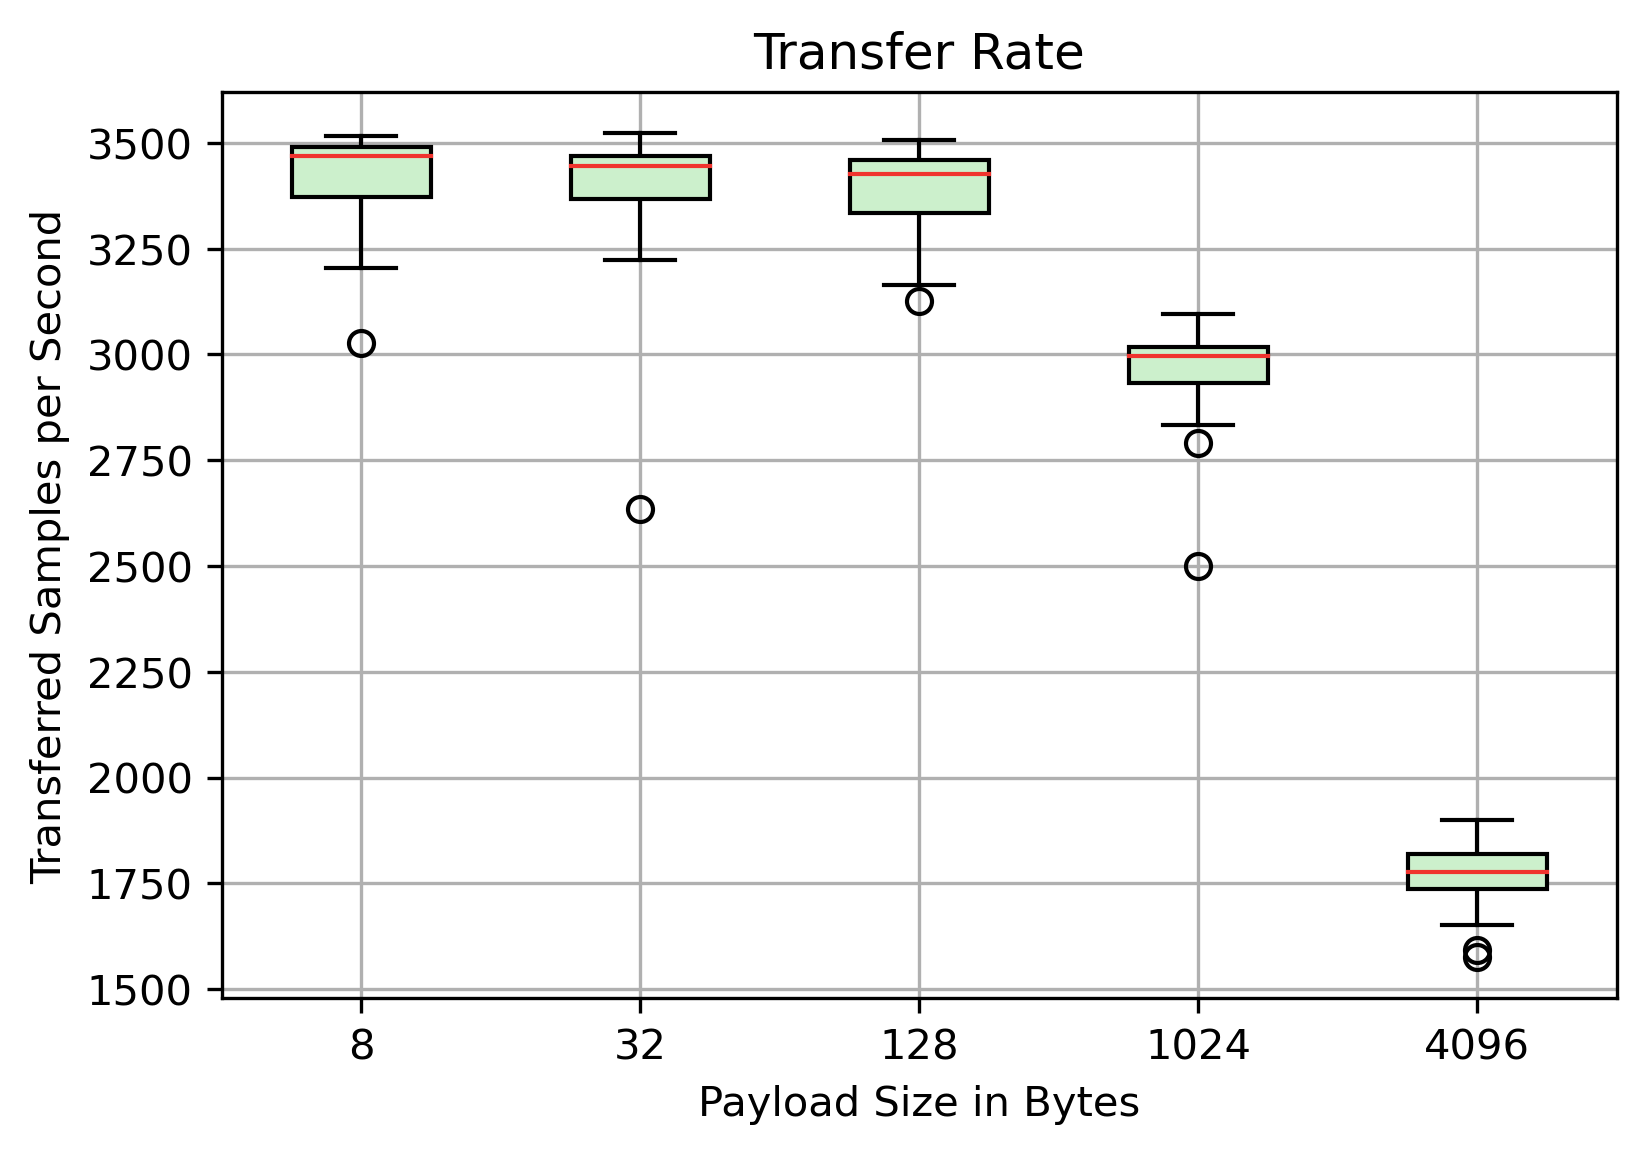
\includegraphics[width=0.8\linewidth]{images/plots/transferRate}
	\caption{The transfer rate of data samples from one replica to another with different payload sizes. As the payload's size increases, the transfer rate decreases.}
	\label{fig:PlotTransferRate}
\end{figure}

\begin{figure}[!htb]
	\centering
	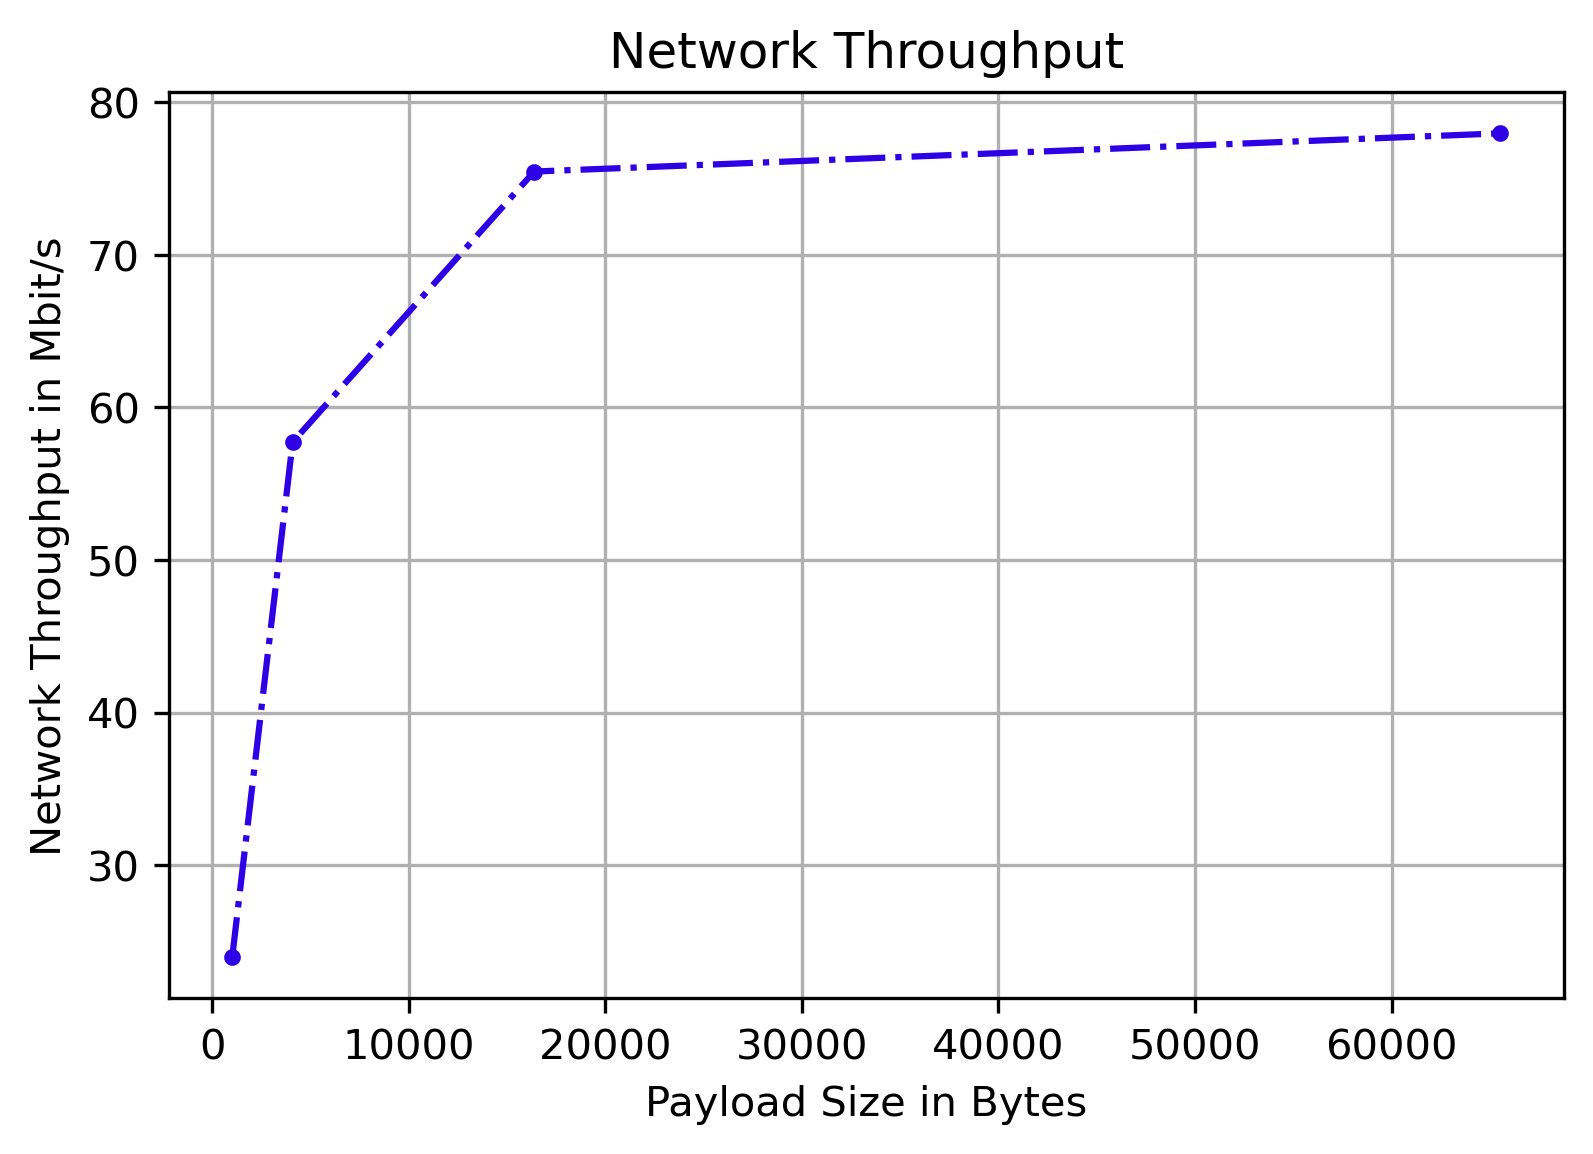
\includegraphics[width=0.8\linewidth]{images/plots/dataThroughput}
	\caption{The average throughput of the network when transferring messages of different sizes from one replica to another. Above a payload size of 15000 bytes, the throughput starts to stagnate due to the \abr{PLC}'s hardware limits.}
	\label{fig:PlotDataThroughput}
\end{figure}

The network's sample transfer rate is depicted in~\autoref{fig:PlotTransferRate}.
While collecting the data, 60 exchanged messages were evaluated.
As the size of sent messages increases, the sample transfer rate decreases.
Whereas an average of 3427~samples per second was transmitted with a payload size of 8 bytes, the average was 1772~samples per second with~4096 bytes.
\\

In another experiment, the network's average data throughput for varying payload sizes was measured.
The results are presented in~\autoref{fig:PlotDataThroughput}.
With a payload size of 1024~bytes, an average data throughput of 24~Mbit/s is reached.
The throughput increases to 56~Mbit/s on average for a payload size of 4096~bytes and 75~Mbit/s on average for a payload size of 16384~bytes.
Above this payload size, the throughput increases less steeply and approaches a value just below 80~Mbit/s.
This value is not far from the 100~MBit/s supported by the \textit{Revolution Pis}' hardware.
\\

Consequently, for payload sized below 4096~bytes, the application and middleware's processing overhead limits the data transmission rate.
For messages with a payload size of 4096~bytes and above, the data transmission is limited by the network's throughput rate.
Because the messages exchanged by replicas in the system are small, results show that the applied resources used are sufficient and the system's safety is not affected by network latency.
\\

As the results show, the communication is stable with only a few outliers.
This work's \abr{QOS}-policies are based on Song \etal~\cite{SongDDSInRealTimeSystems}.
Although Song \etal utilized a different \abr{DDS} implementation and used a different processing hardware, their network characteristics are the same.
Compared to Song \etal the communication of this work's system is a little slower.
While they reached a latency of around 280 microseconds for one kilobyte of data, the proposed architecture reached around 330 microseconds for a one-kilobyte payload.
However, the values are similar so that the real-time capability of \abr{DDS} - shown by Song \etal - can be transferred to the architecture studied here.


\subsection{Resource Utilization}

The PLCs that were utalized in this work were chosen as a simple model.
However, this model is relevant to a real-world rail scenario with comparable low-cost rail controllers.
Thus, the system is intended to operate on small and \abr{COTS} \abrpl{PLC} where resources are limited.
However, it operates in a time-critical environment in which the lack of available resources should not affect execution.
The utilization was measured in idle mode and while processing scenarios to make statements about resource utilization and differentiate between fundamental- and productive utilization.
Measurements were made with \textit{pidstat}, a tool that monitors individual tasks that are managed by the \abr{OS} kernel.
In this section, the resource utilization for both the leader replica and the follower replicas are analyzed.
At first, the \abr{CPU} utilization is considered, then the memory consumption.

\paragraph{Idle Mode CPU Utilization}

\begin{figure}[!hbt]
	\centering
	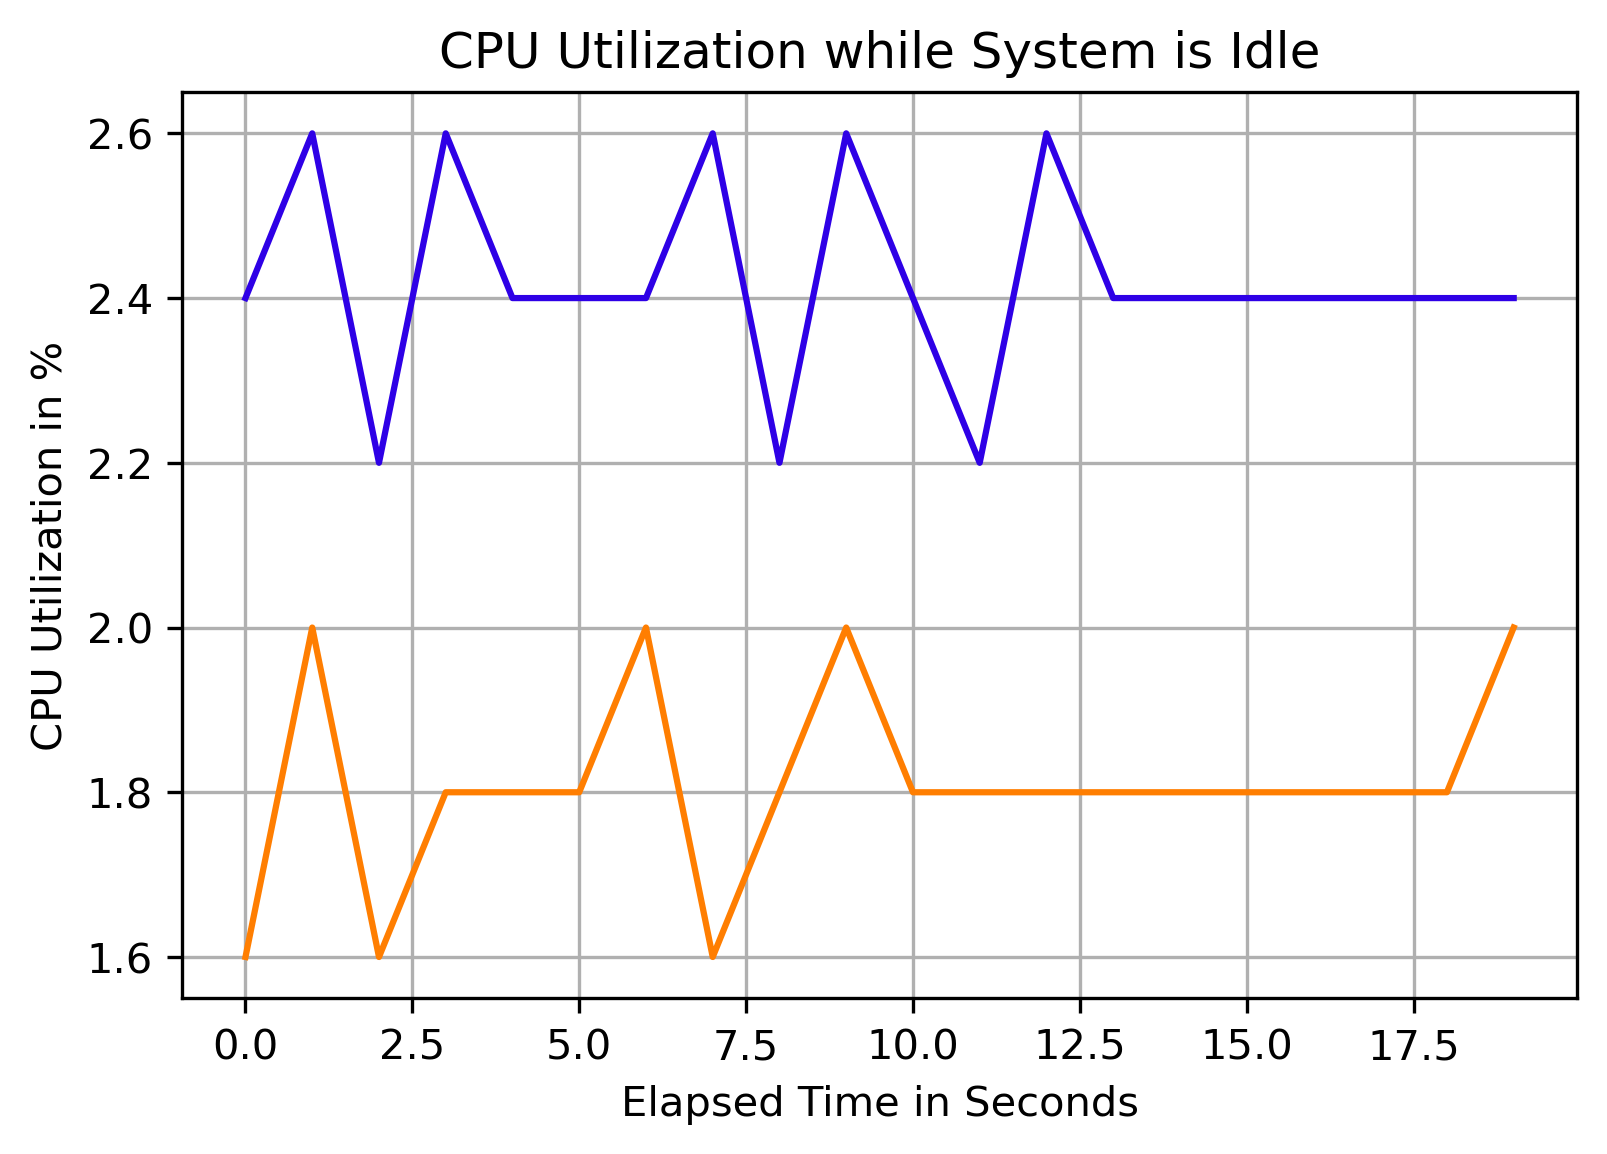
\includegraphics[width=0.8\linewidth]{images/plots/CPUUsageIdleTime}
	\caption{In idle mode, only heartbeat messages are transmitted from the leader to its followers. Hence, the leader's \abr{CPU} is more demanded, but the overall utilization is below 3\%.}
	\label{fig:PlotCPUUsageIdleTime}
\end{figure}


In idle mode, the train is not driving and only heartbeat messages are exchanged between the leader and its followers.
The idle mode \abr{CPU} utilization for both a leader and a follower is depicted in~\autoref{fig:PlotCPUUsageIdleTime}.
Results show that the leader's idle \abr{CPU} utilization is consistently higher than the follower's.
On average, the follower utilized 1.81\% in 90 seconds, while the leader utilized 2.42\% of the applied \abr{CPU}.
At system-mode, 0.21\% are used for the leader and 0.25\% for a follower on average.
On user-mode, the leader utilizes on average 1.0\%, while a follower uses 0.66\%.
This can be explained by the fact that the leader has more responsibilities in idle mode.
It periodically sends heartbeat messages and observes whether the train has a valid \abr{MA} and can start driving.


\paragraph{CPU Utilization during Journey}

During a journey, the system monitors the state of the train and evaluates input messages.
To measure the resource utilization in different situations, the three test scenarios were executed one after the other.
The beginning of the first scenario - \texttt{Reach End of MA} - is marked by \textbf{S1}.
The beginning of \texttt{Unlinked Balise} is marked with \textbf{S2} and the beginning of \texttt{Balise not where expected} with \textbf{S3}.

\begin{figure}[!htb]
	\centering
	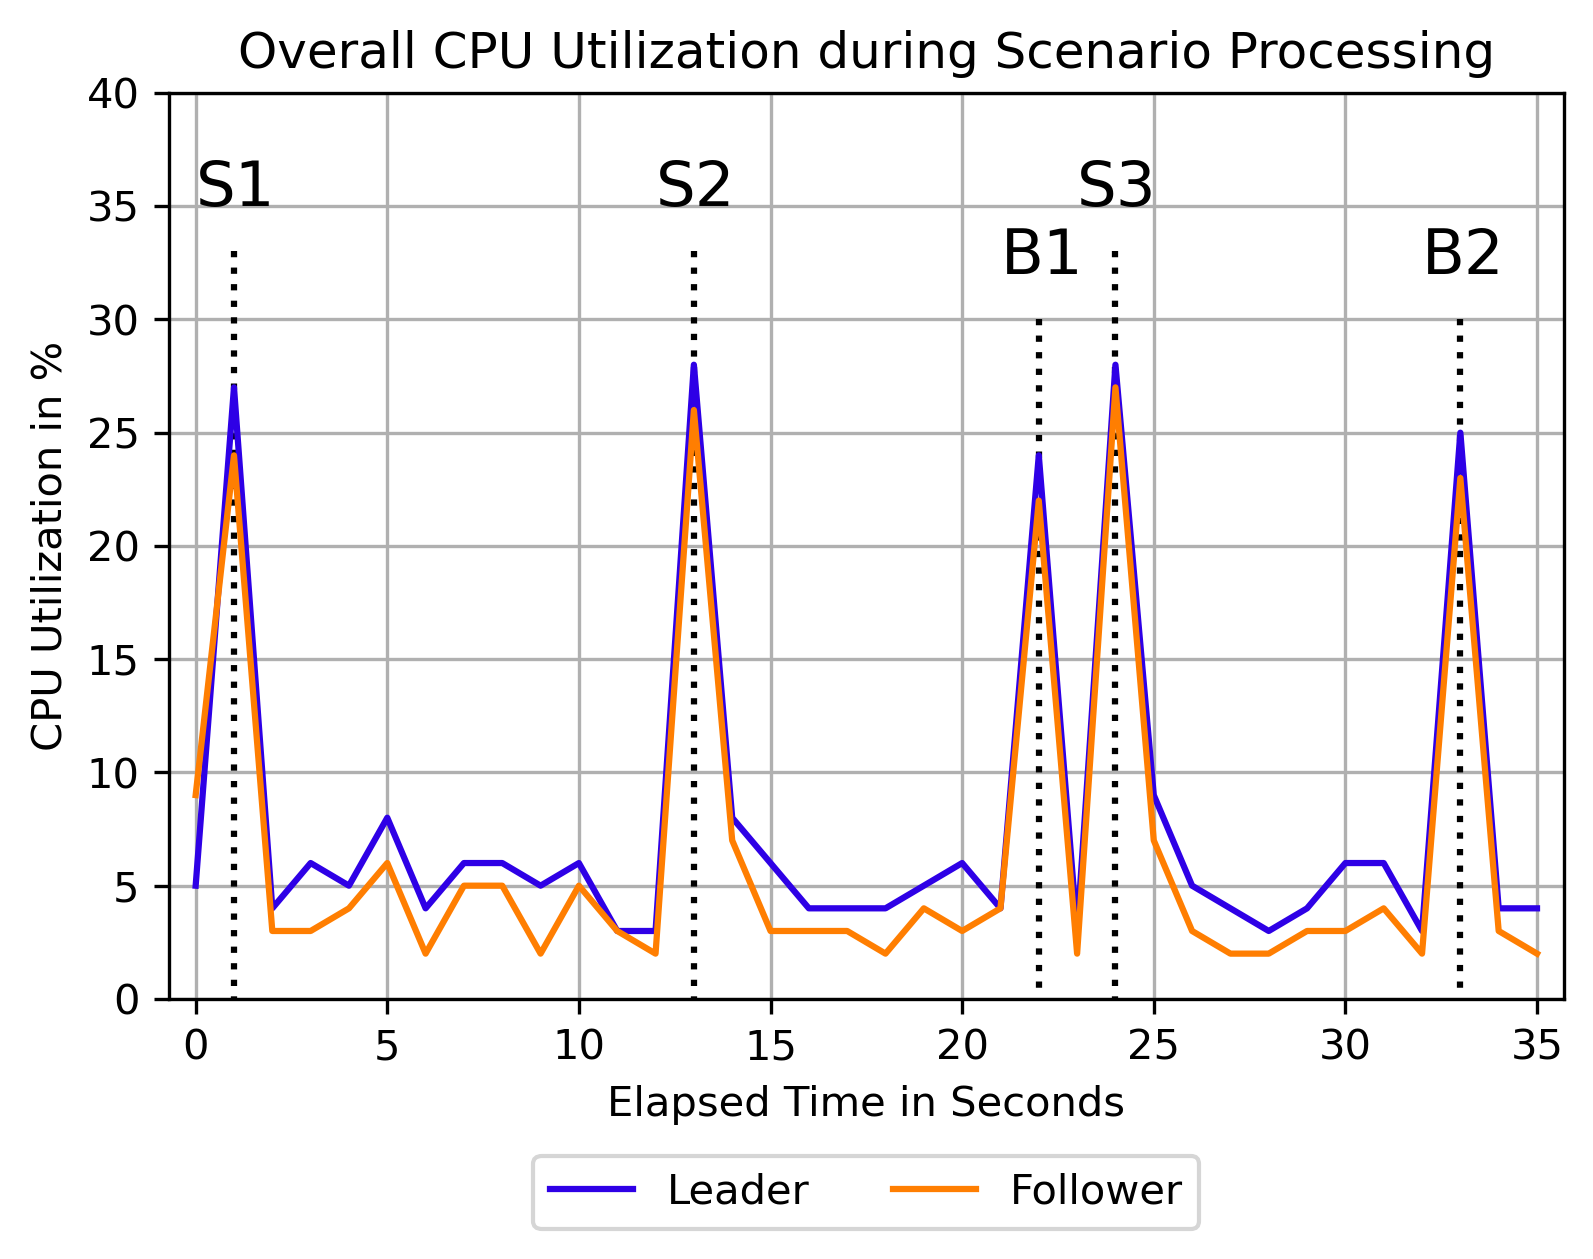
\includegraphics[width=0.8\linewidth]{images/plots/TotalCPUUsage}
	\caption{\abr{CPU} utilization during a train's journey. Three scenarios are processed one after the other. At \textbf{S1}, \textbf{S2}, and \textbf{S3} the individual scenarios start with the reception of \abr{MA} and linking information which is shared among replicas via the global system state. At \textbf{B1}, an unlinked balise was encountered. At \textbf{B2}, a balise was received whose position does not correspond with its linked position. In both cases, the train has to brake before arriving at the \abr{MA}'s end.}
	\label{fig:PlotTotalCPUUsage}
\end{figure}

An overview of the total \abr{CPU} utilization while processing the scenarios is presented in~\autoref{fig:PlotTotalCPUUsage}.
The total \abr{CPU} utilization reflects different situations that happen during the journey.
At the beginning of each scenario, both the leader and the follower show a peak (\textbf{S1}, \textbf{S2}, and \textbf{S3}).
This is because the leader evaluates the transmitted \abr{MA} and the set of linked balises, publishes them to the global state and starts simulating the train.
The middleware on the follower side registers, receives, and processes the new state.
During the journey, where the braking curve is constantly monitored, the utilization fluctuates around 5\%.
The remaining two peaks are due to premature brakings.
At \textbf{B1}, an unlinked balise is noticed by the system and at \textbf{B2}, a balise at an unexpected location is received.

\begin{figure}[!hbt]
	\centering
	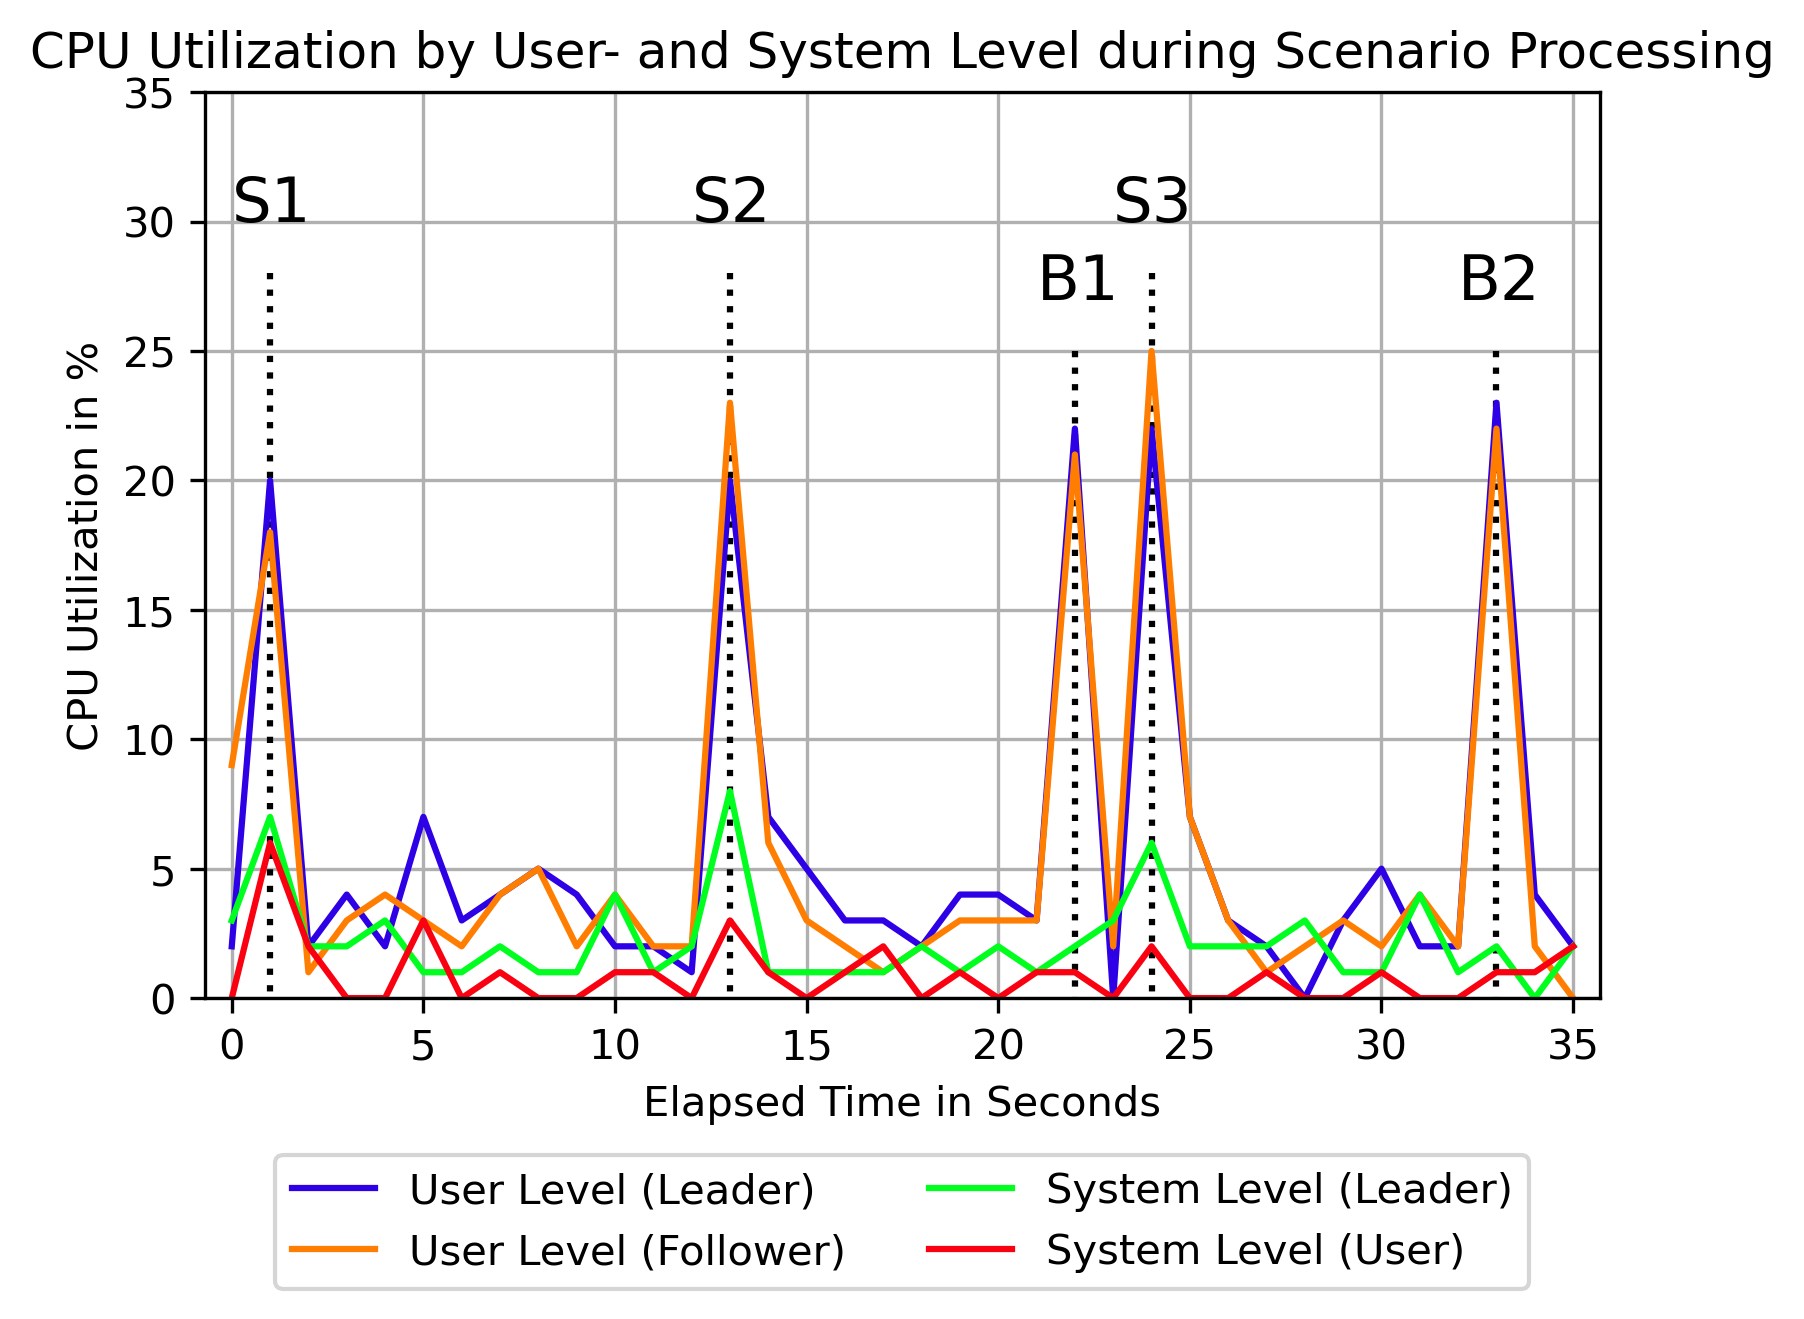
\includegraphics[width=0.8\linewidth]{images/plots/SystemUserCPUUsage}
	\caption{Most of the \abr{CPU} work is done at user-mode. When \abr{MA} and linking information are received (\textbf{S1}, \textbf{S2}, and \textbf{S3}) peaks occur on both user- and system-mode. However, the leader performs more work on system-mode than the followers. This can be explained by the fact that memory is requested for the new state information. For early braking situations (\textbf{B1}, and \textbf{B2}), work is mostly done at user-mode and the system-mode utilization shows no peaks here.}
	\label{fig:PlotSystemUserCPUUsage}
\end{figure}

In~\autoref{fig:PlotSystemUserCPUUsage}, a distinction is made between \abr{CPU} utilization at user-mode and at system-mode.
It can be seen that the application operates mainly at user-mode.
At the beginning of each journey, when \abr{MA} and linking information are received, peaks on system-mode occur (\textbf{S1}, \textbf{S2}, and \textbf{S3}).
The peaks on system-mode utililzation are mainly on leader side and can be explained by the fact that new instances in the global state are created for the new information.
The peaks on user-mode are due to replica synchronization and simulation start.
In case of a premature stop (\textbf{B1} and \textbf{B2}), the calculation is almost exclusively done at user-mode in order to synchronize the replicas and stop the simulation.

\paragraph{Memory Consumption}
The memory consumption is constant both in idle mode and when processing the scenarios.
In idle mode, 10.5~MBit were used from both the leader and the follower.
It increases to 11.2~MBit while scenarios are processed.
This can be explained by the fact that the supplied \abr{MA} and the linked balises are stored.
Further, additional messages are exchanged between the replicas.
The memory consumption is constant during the whole time due to the chosen approach where all memory is allocated at program startup.


\subsection{Leader Election}
\label{subsec:LeaderElectionEval}
\begin{figure}[!htb]
	\centering
	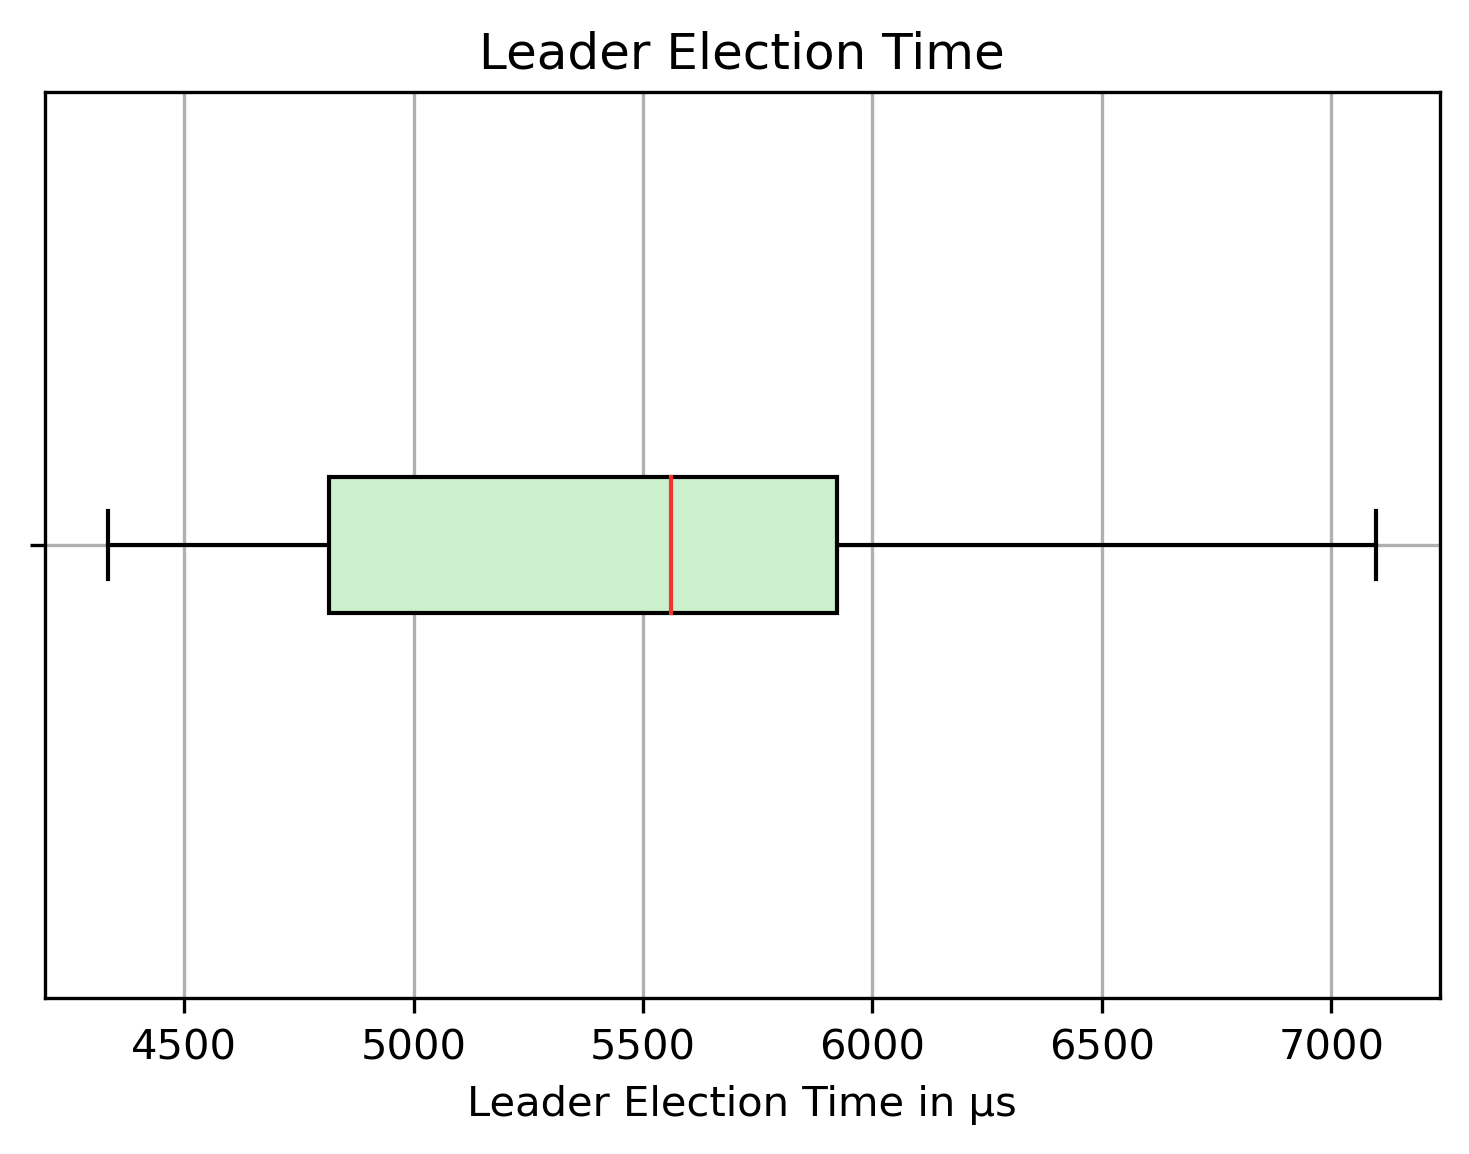
\includegraphics[width=0.8\linewidth]{images/plots/timeWithoutLeader}
	\caption{Leader election time is the time that passes from the point where a missing leader is recognized until the first heartbeat message is sent by the new leader. Data from 20 elections were used for the measurement.}
	\label{fig:PlotTimeWithoutLeader}
\end{figure}

When the system notices the absence of a leader, a new one gets elected.
In the following, the maximum time the system can be without a leader is determined.
\\

A leader communicates its existence to the remaining replicas via heartbeat messages.
The lower limit of the time that the system is without a leader after the previous leader failed is regulated by the \textit{election timeout}.
In addition, time is required for the election process itself.
The leader election process consists of requesting and collecting votes from all replicas in the system.
An election process' duration is influenced by the replica's computational resources and data transmission speed.
In order to investigate how long the leader election process takes, the time for 20 elections was measured.
The average time for an election process is depicted in~\autoref{fig:PlotTimeWithoutLeader}.
Results show that the election process takes 5.5~ms on average and at worst 7.1~ms.
\\

Under special circumstances, it may be impossible for the system to elect a leader.
This can, for example, be the case when there are not enough replicas in the system to reach a majority.
For this case, another timeout is used, called \textit{leader ready timeout}.
This timeout determines the maximum time that a candidate waits for incoming votes.
After a selectable number of failed elections, the election process gets aborted and a braking process is initiated.
\\

Recapped , the maximum time that the system can typically be without a leader is determined by the \textit{election timeout} plus the election time.
When a leader election is impossible, the maximum time is determined by the \textit{election timeout} plus the \textit{leader ready timeout} times the number of allowed failed elections.

\subsection{Scenario Processing}

During its journey, the on-board system periodically monitors the train's state and handles input messages.
While doing so, the participating replicas exchange messages.
All communication originates from the system's leader, that makes requests and receives responses from the remaining replicas.
Based on the chronology of the exchanged messages, the system's behavior in different situations can be comprehended and analyzed.
Therefore, the three test scenarios are simulated one after the other.
In the following plots, the beginning of the first scenario - \texttt{Reach End of MA} - is marked by \textbf{S1}.
The beginning of \texttt{Unlinked Balise} is marked with \textbf{S2} and the beginning of \texttt{Balise not where expected} with \textbf{S3}.
Before the third scenario is started, the previous leader was manually stopped at the moment labeled with \textbf{LC}.
%Without manually stopping the leader, the system ran for 60 minutes without reelection.
%After 60 minutes, the processing was manually stopped.

Any active hardware redundancy mechanisms have been disabled at first.
Thus, the third scenario has been run only with a leader and one follower, instead of a leader and two followers in the first two scenarios.
Later, the active hardware redundancy features are reactivated to show their benefits on the system's reliability.
For each measurement, the heartbeat timer has been set to 100~ms so that ten messages per second can be attributed to heartbeat messages.
\\

At first, the number of received input messages is presented and the processing time for each input is measured to show that no input is lost.
Then, the total number of sent messages by all replicas are examined and put into a ratio between leader and follower.
Afterward, the sent and received messages are analyzed for event-, as well as state topics.
This provides insight into how the system handles inputs and shows how component failures impact the system's behavior.
Finally, another run is made, this time with an active spare unit.
Therefore, the received events are measured to show how a spare increases the system's reliability.

\paragraph{Input Messages}

\begin{figure}[!hb]
	\centering
	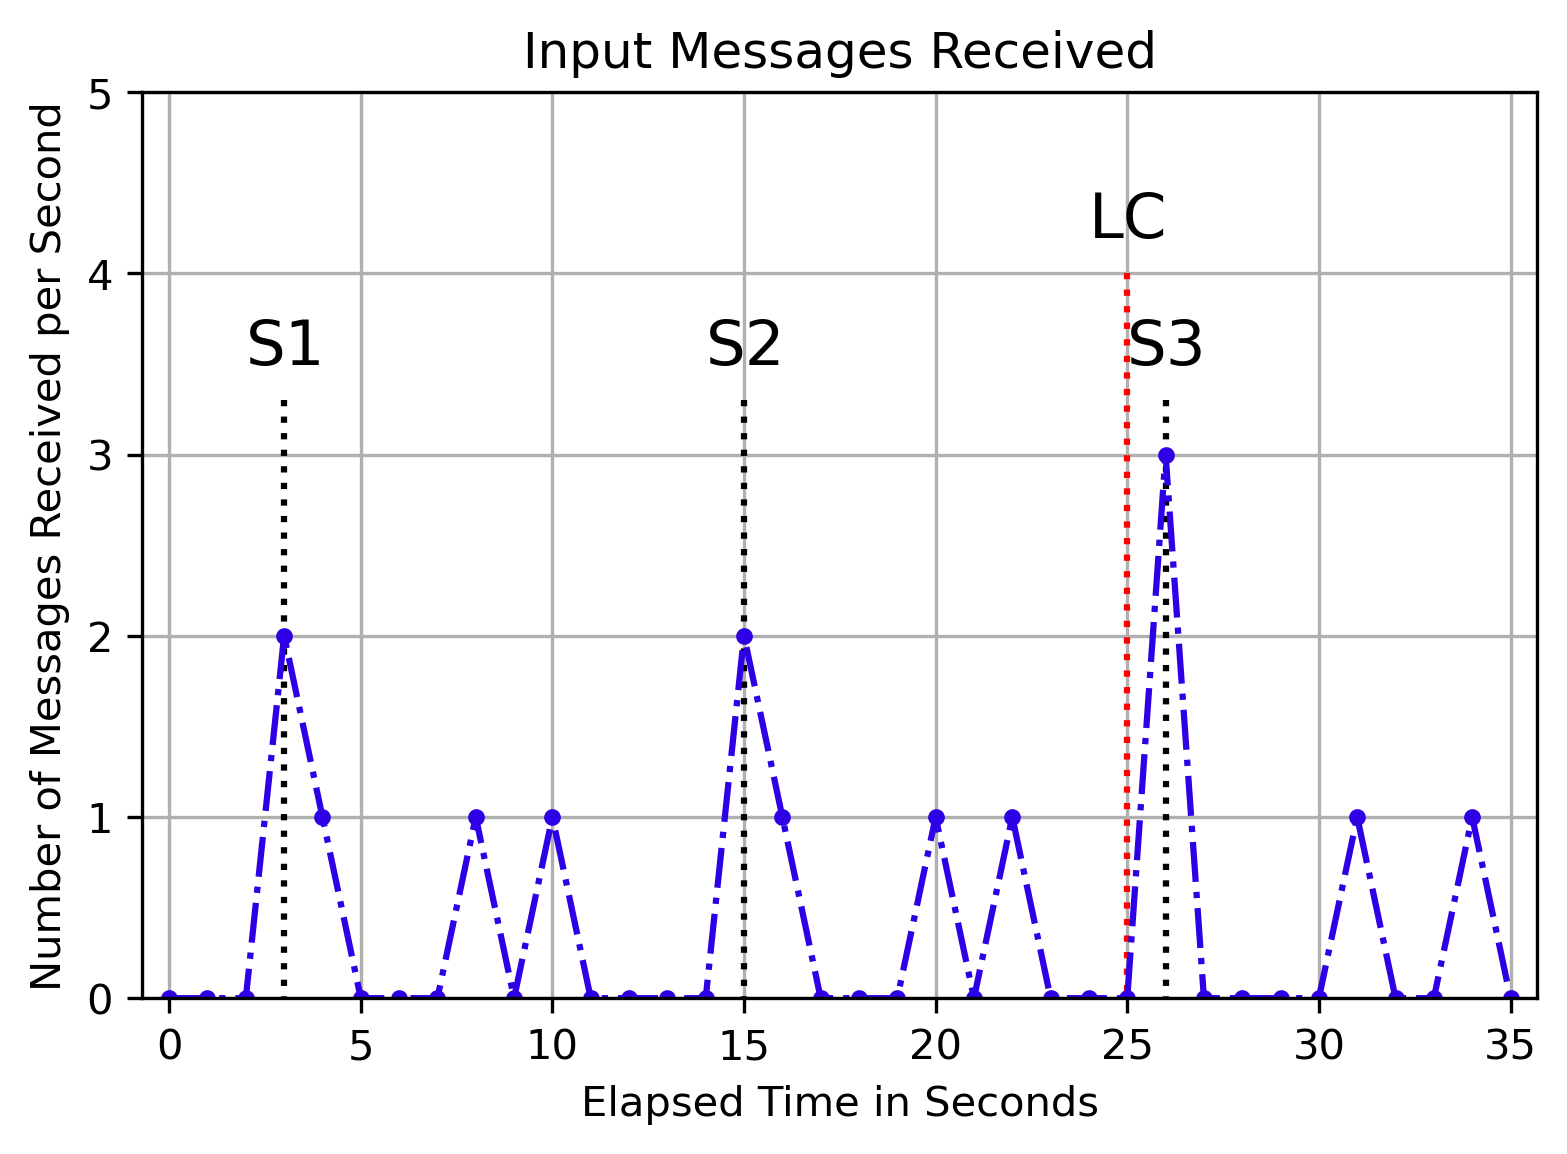
\includegraphics[width=0.8\linewidth]{images/plots/InputMessagesReceive}
	\caption{Number of input messages that the system receives throughout three scenarios. The first scenario starts after three seconds (\textbf{S1}), the second after 15 seconds (\textbf{S2}), and the third after 26 seconds (\textbf{S3}). After 25 seconds, the previous leader was manually stopped (\textbf{LC}). The peaks at \textbf{S1} and \textbf{S2} indicate that one message with \abr{MA} and one with linking information was received. At \textbf{S3}, three input messages are received. This is because the \abr{MA} and linking message were buffered until a new leader got elected. The remaining peaks indicate that balise telegrams were received.}
	\label{fig:PlotInputMessagesReceive}
\end{figure}

The individual scenarios' structures can be traced by the input messages that the system receives.
This is depicted in~\autoref{fig:PlotInputMessagesReceive}.
At the beginning of each scenario, one message with the \abr{MA} and one with the linked balises are received.
Then, during each scenario, three balise telegrams are obtained.
While the \abr{MA} and linking information are received before the first balise telegram for the first two scenarios, they are taken at once for the third scenario.
This is due to the previously crashed leader.
However, it further shows that the input messages are buffered and no input message is lost, even if the leader crashed right before input is received.
\\

Response times and availability for \texttt{Raft}-based consensus systems have been studied by Sakic and Kellerer~\cite{SakicTimeInConsensus}.
Their results show that in a cluster with three components, each event can be handled in at least 1000~ms.
The event processing time for this work's application depends on two factors; the presence of a leader and the input processing time.
In a worst-case - in which the leader fails while a new input event occurs - the absent leader needs to be recognized, a new one needs to be elected, and the input needs to be processed.
Since leader election and input processing times are small, the \textit{election timeout} is the decisive factor.
With an \textit{election timeout} of 500~ms, the system guarantees a result after around 600~ms.
The result is suitable for \abr{ETCS} applications whose demands for on-board units include a maximal reaction time of 1000~ms~\cite{ETCS26}.


\begin{figure}[!hb]
	\centering
	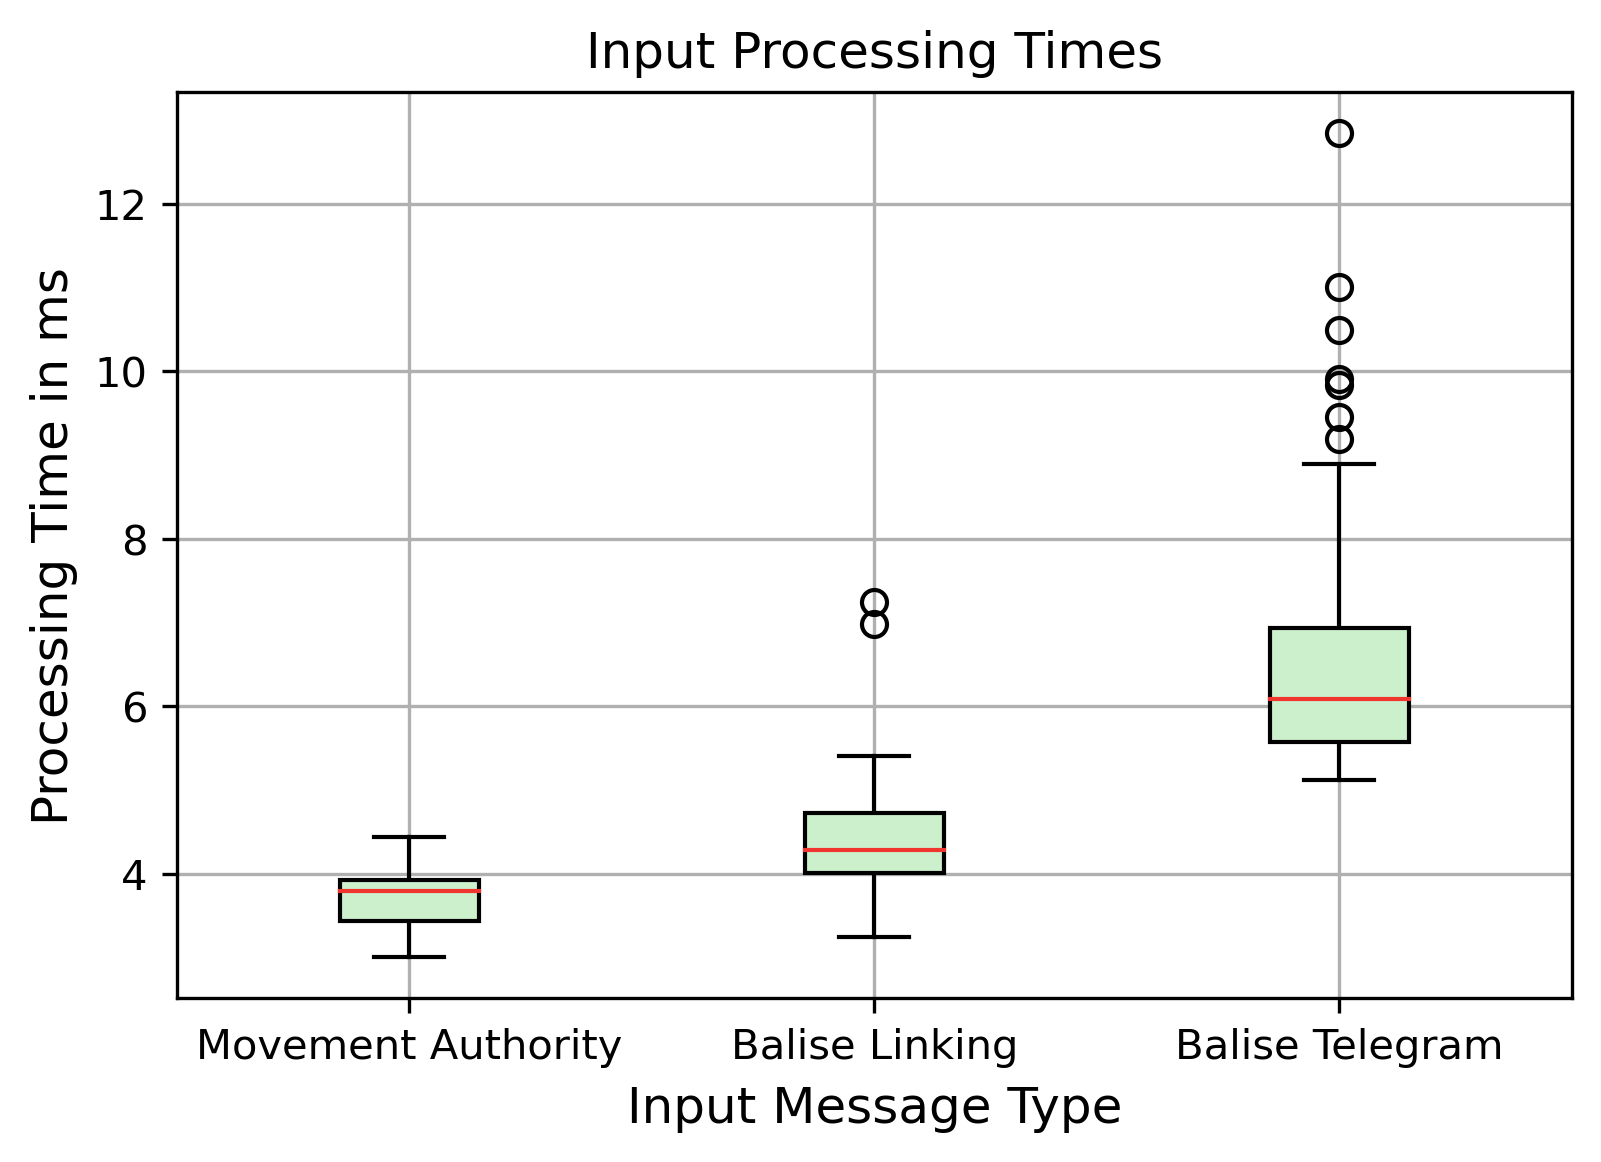
\includegraphics[width=0.8\linewidth]{images/plots/inputProcessingTimes}
	\caption{Time it takes the system to process input messages of different types. The \texttt{Movement Authority} and \texttt{Balise Linking} input type require the leader to add data to the system's global state. A linking message includes more data and therefore requires more time. For messages of \texttt{Balise Telegram} type, the system performs redundant computation and final voting. The outliers are due to balise telegrams that require the operated train to brake, such as an unlinked balise.}
	\label{fig:PlotInputProcessingTimes}
\end{figure}

The inputs are processed differently by the system depending on the information they contain.
An overview about processing times for different input message types is shown in~\autoref{fig:PlotInputProcessingTimes}.
\abr{MA} and balise linking telegrams are read by the leader and published to the systems' global data space.
Unlike balise telegrams, no system-wide and redundant decision-making is required.
Upon receiving a balise telegram, the leader requests decisions from its followers and performs a final voting.
Therefore, network latency, message processing, and voting add to the overall balise telegram processing time.

\paragraph{Total Messages}

\begin{figure}[!hb]
	\centering
	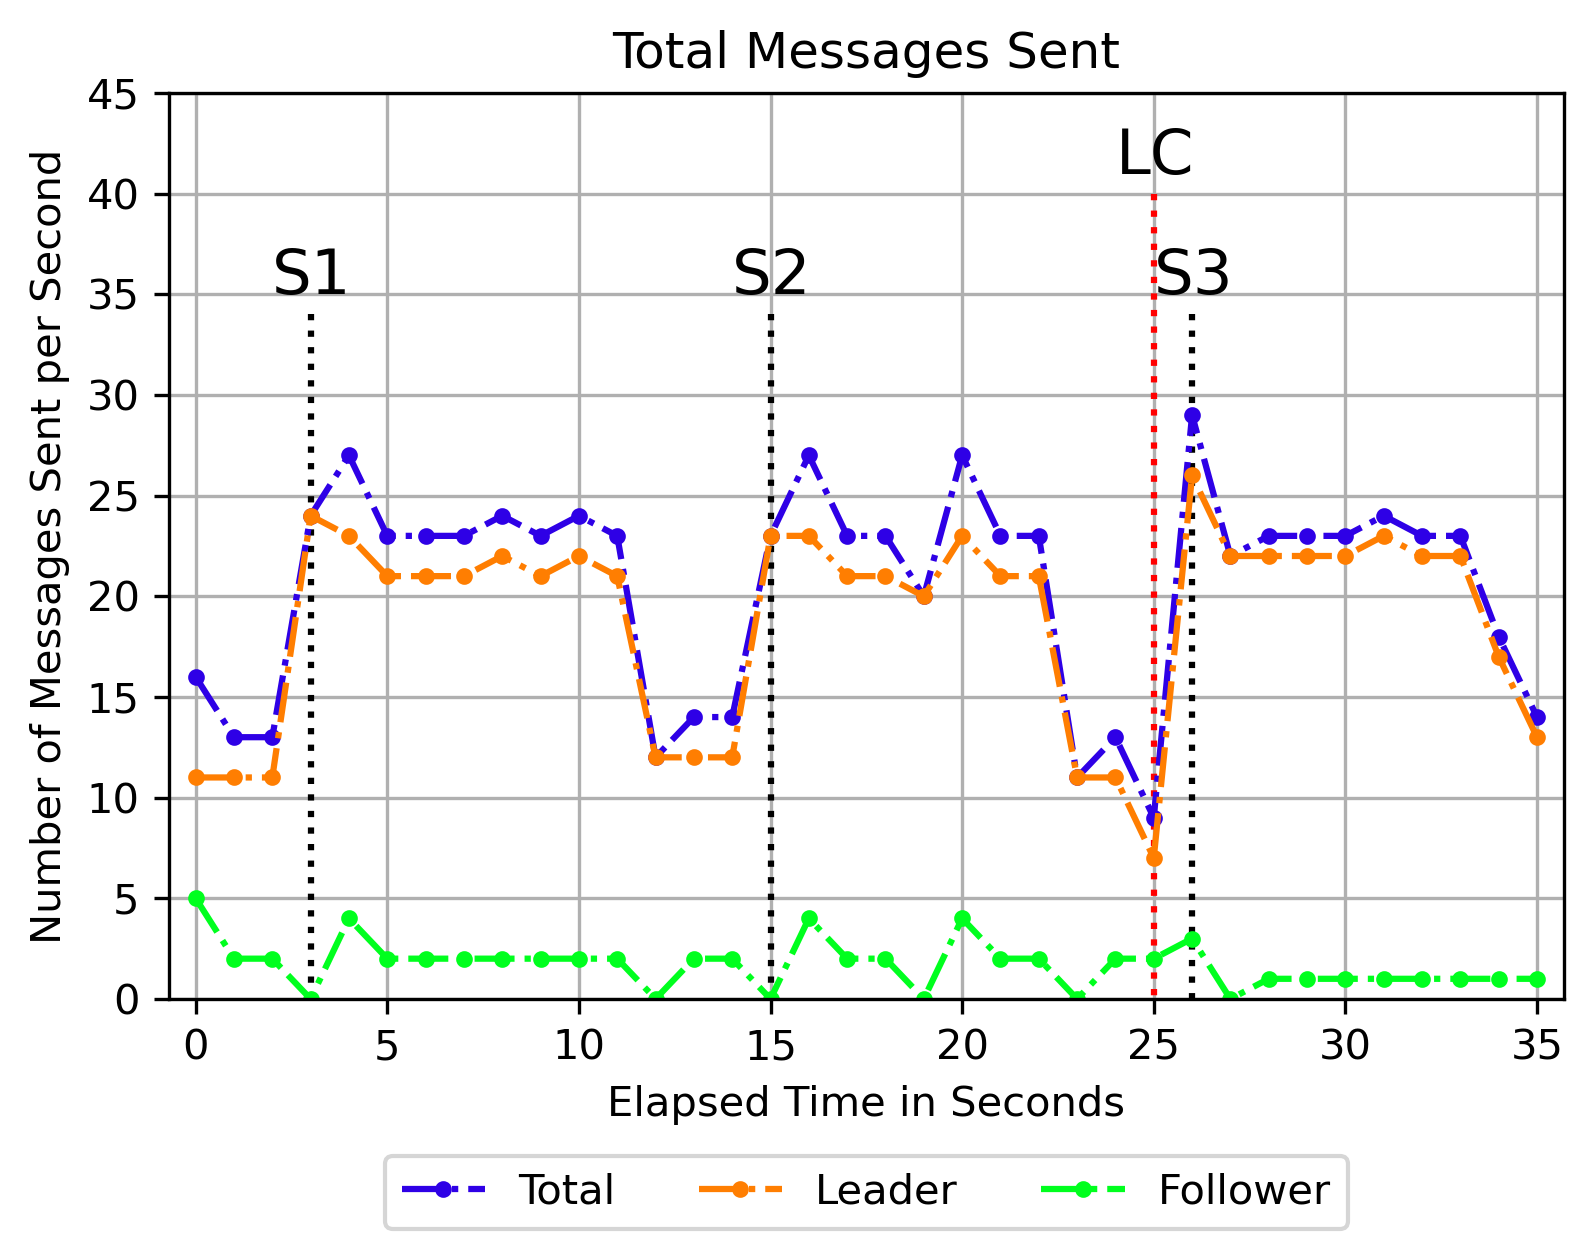
\includegraphics[width=0.8\linewidth]{images/plots/TotalMessagesSent}
	\caption{All messages that were published by replicas over a period of three scenarios that start at \textbf{S1}, \textbf{S2}, and \textbf{S3}. After 25 seconds, the system's leader was manually stopped (\textbf{LC}). The number of messages sent after the first leader stopped does not differ from those sent before, showing the system's robustness.}
	\label{fig:PlotTotalMessagesSent}
\end{figure}

The total number of messages sent per second by the replicas is shown in~\autoref{fig:PlotTotalMessagesSent}.
The beginning and end of each of the three scenarios can be seen in the plot by the total number of sent messages.
While the train is driving, 20-25 messages are sent per second.
The number reduces to 12-14 after a scenario finished, the train stoped, and the system returned to idle mode.
While the train is driving, it is the leader's responsibility to update the system's global state, explaining the prominent increase in sent messages during operation.
A majority of messages are sent by the system's leader, ten alone due to heartbeat messages.
The rest accrue from a system-wide braking curve monitoring, for which requests and responses are transmitted.
The robustness of the system is shown by the fact that the number of messages sent for the last scenario (\textbf{S3}) - after the previous leader stopped (\textbf{LC}) - does not differ from the previous two scenarios.

\paragraph{State Messages Sent}

\begin{figure}[!htb]
	\centering
	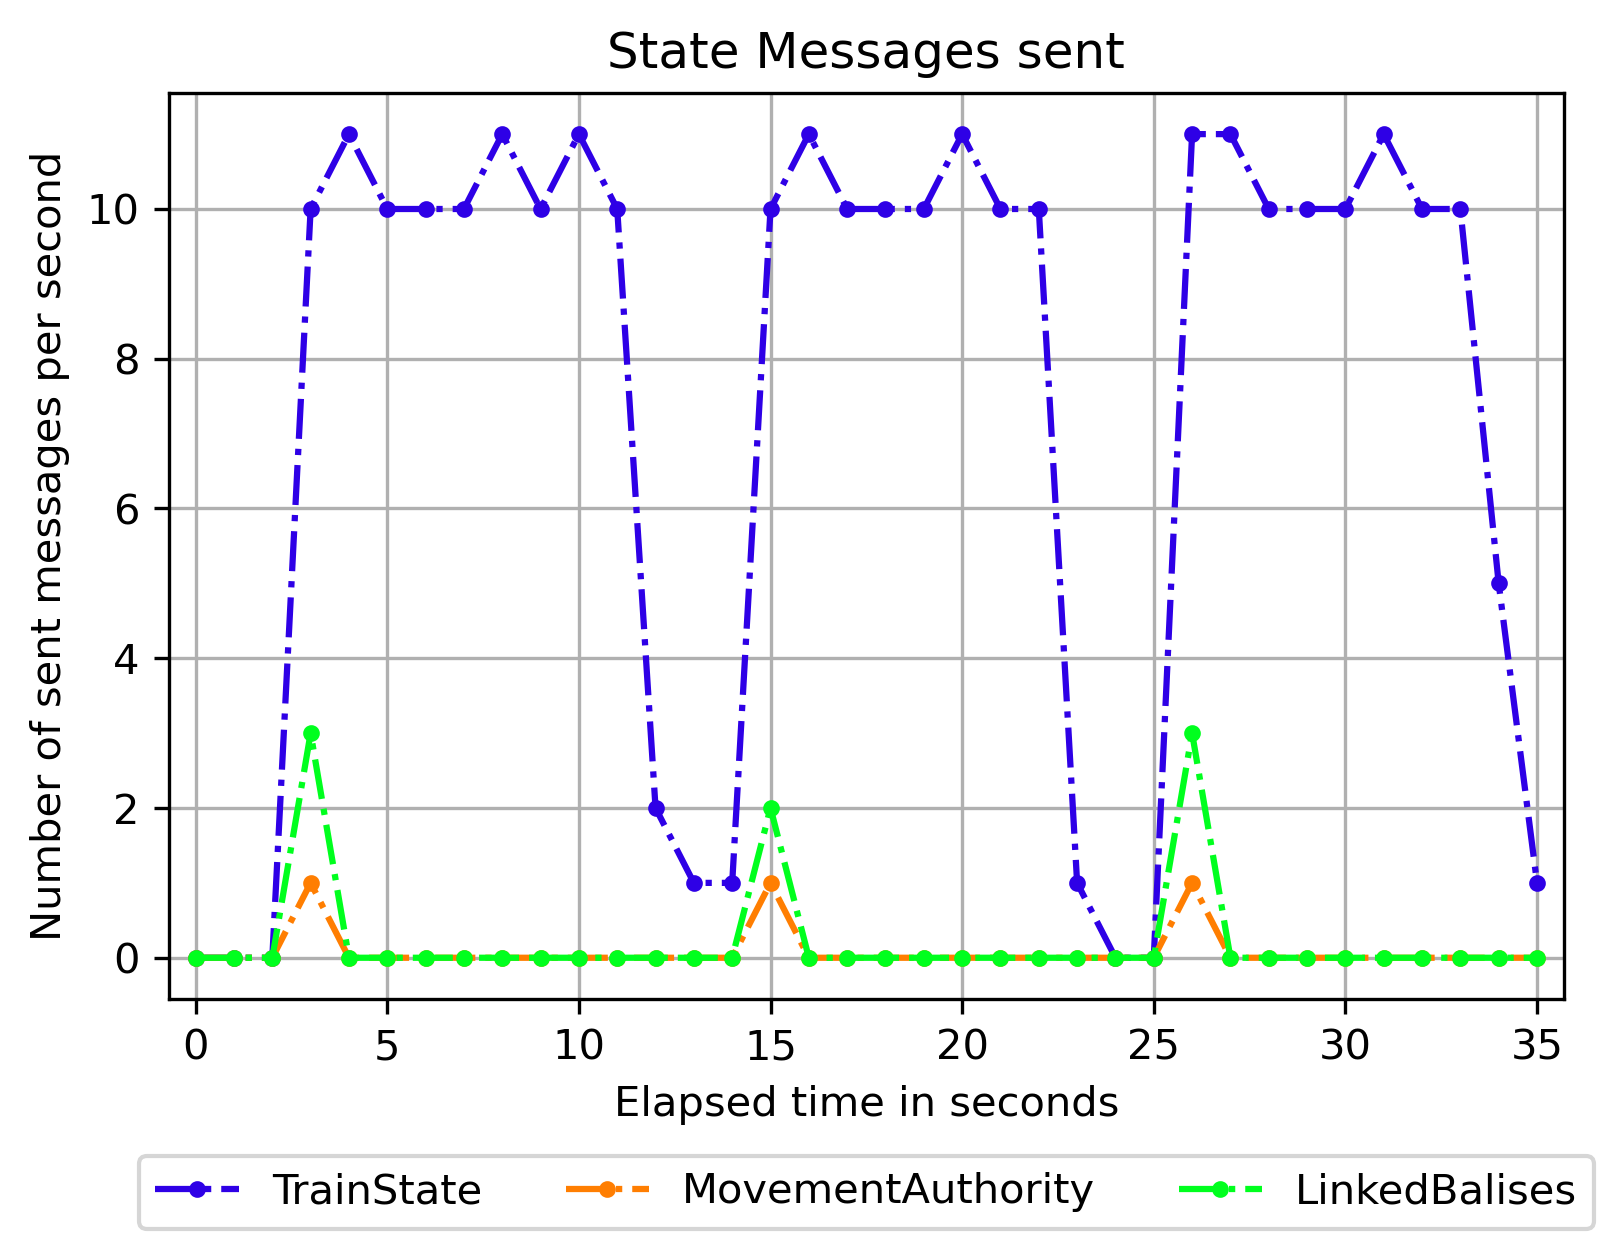
\includegraphics[width=0.8\linewidth]{images/plots/StateMessagesSent}
	\caption{Messages that were published to state topics over a period of three scenarios that start at \textbf{S1}, \textbf{S2}, and \textbf{S3}. For the first and third scenario, three balises were linked. The second balise includes an unlinked balise and therefore, only two are linked. Further, a crashed leader (at point \textbf{LC}) does not affect the system state's up-to-dateness.}
	\label{fig:PlotStateMessagesSent}
\end{figure}

State topics include \texttt{TrainState}, \texttt{MovementAuthority}, and \texttt{LinkedBalises}.
The number of messages published to these topics can be seen in~\autoref{fig:PlotStateMessagesSent}.
It is noticeable that most state messages are published on the \texttt{TrainState} topic.
This is because the position is simulated every 100~ms and written to \texttt{TrainState}.
Messages to \texttt{MovementAuthority} and \texttt{LinkedBalises} are only published at the beginning of each scenario because, at this time, the \abr{MA} and linked balises are communicated to the system.
It can further be seen that three balises are linked in the first and third scenario, but only two linked balises are added for the second.
The state messages are all sent by the leader because it is the only replica allowed to publish to these topics.
After the previous leader stopped (\textbf{LC}), messages are still published to the state topics.
Hence, a new leader has been elected.

\paragraph{Behavioral Messages}

\begin{figure}[h!]
	\centering
	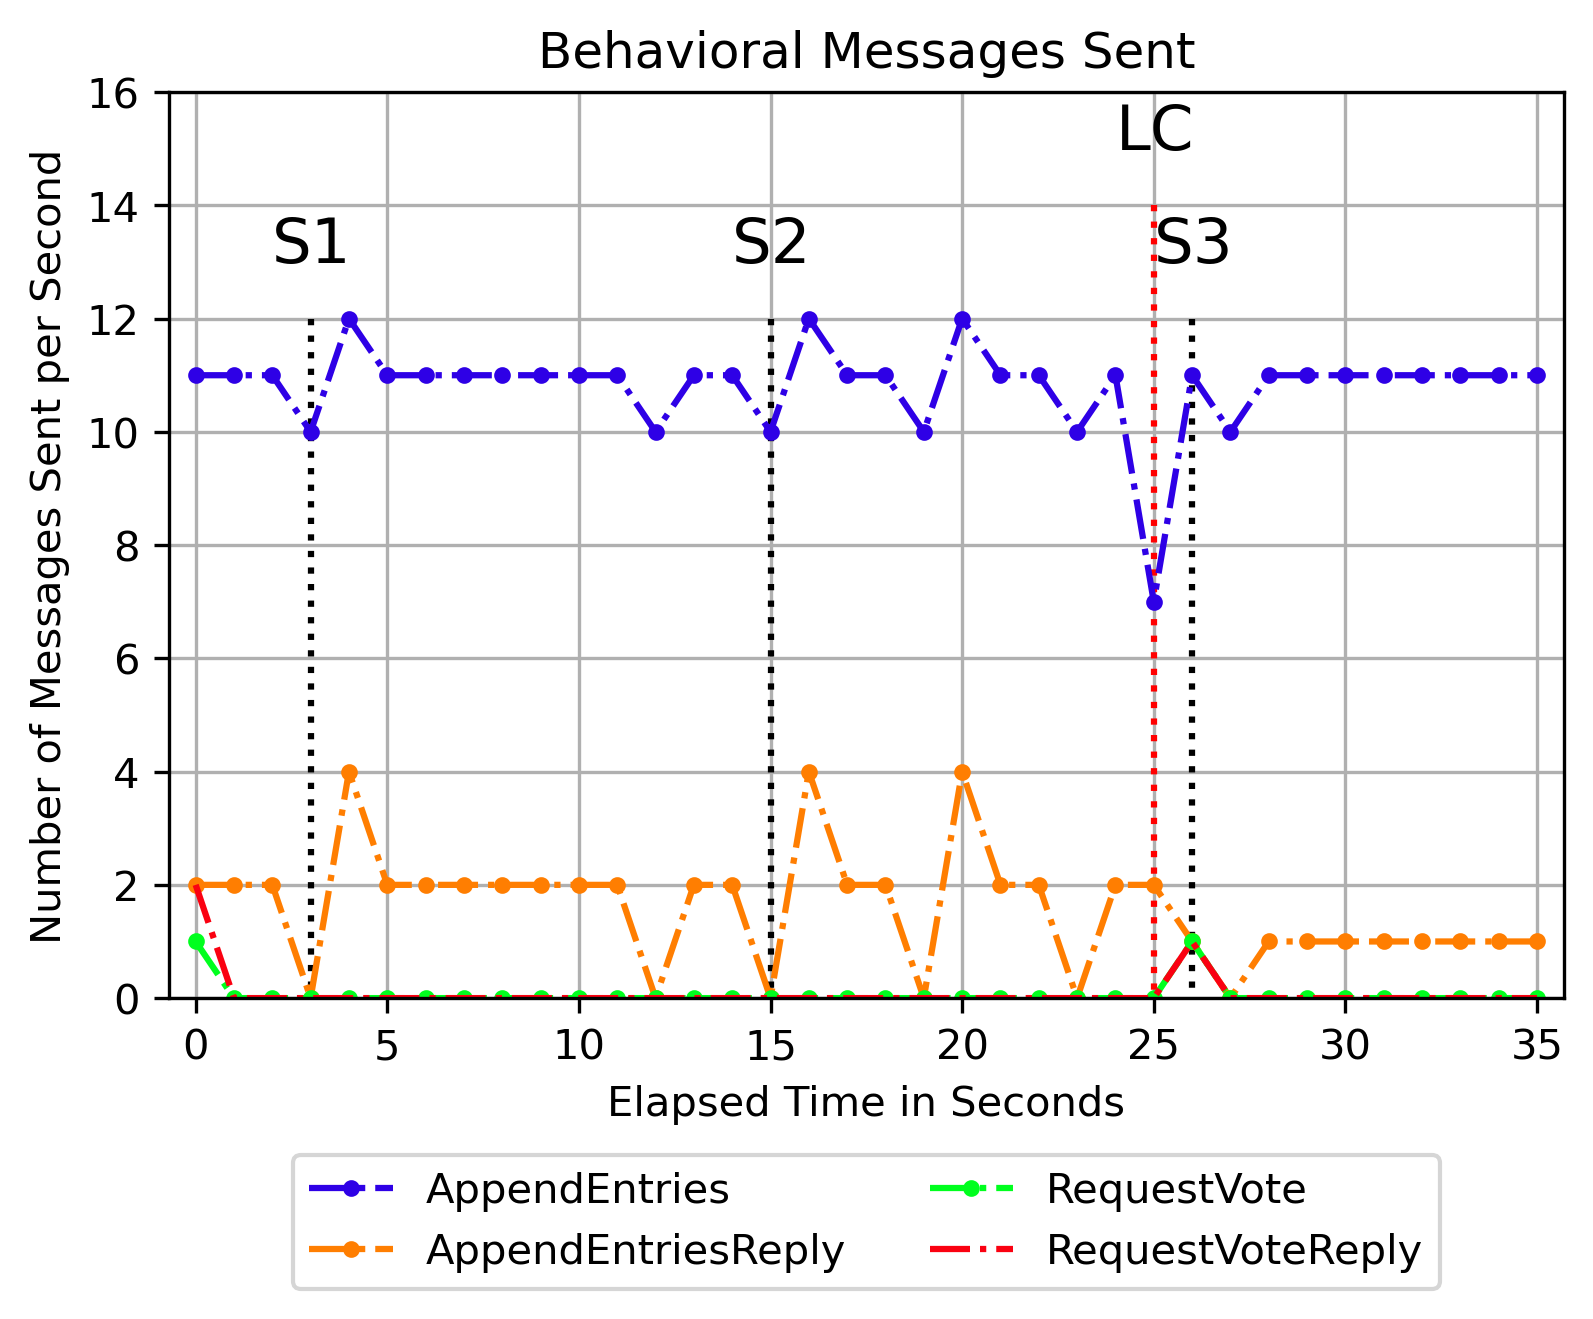
\includegraphics[width=0.8\linewidth]{images/plots/ConsensusMessagesSent}
	\caption{The number of messages that were published to behavioral topics throughout three scenarios that start at \textbf{S1}, \textbf{S2}, and \textbf{S3}. As soon as the first leader stopped (at point \textbf{LC}), the number of heartbeat messages on the \texttt{AppendEntries} topic decreases. The leader crash is followed by a leader election - a message being sent on \texttt{RequestVote} and \texttt{RequestVoteReply}. Afterward, the number of heartbeat messages goes back to the previous value showing that a new leader got elected.}
	\label{fig:PlotConsensusMessagesSent}
\end{figure}

Behavioral topics include \texttt{AppendEntries}, \texttt{AppendEntriesReply}, \texttt{RequestVote}, and \texttt{RequestVoteReply}.
The majority of messages is published to the \texttt{AppendEntries} topic due to the leader periodically publishing heartbeat messages.
Before the first scenario is executed, a leader election takes place which is indicated by traffic on \texttt{RequestVote} and \texttt{RequestVoteReply}.
Another leader election happens after the previous leader crashed (\textbf{LC}).
The fact that the previous leader crashed is reflected in the collapse of heartbeat messages on the \texttt{AppendEntries} topic.
Again, a vote request is published to the corresponding topic by the first replica that notices the absent leader.
This time, only one vote reply is published because only one other replica remains in the system.
The fact that the amount of heartbeat messages increases back to the number before the first leader crashed indicates that a new leader has been established.


\begin{figure}[!hb]
	\centering
	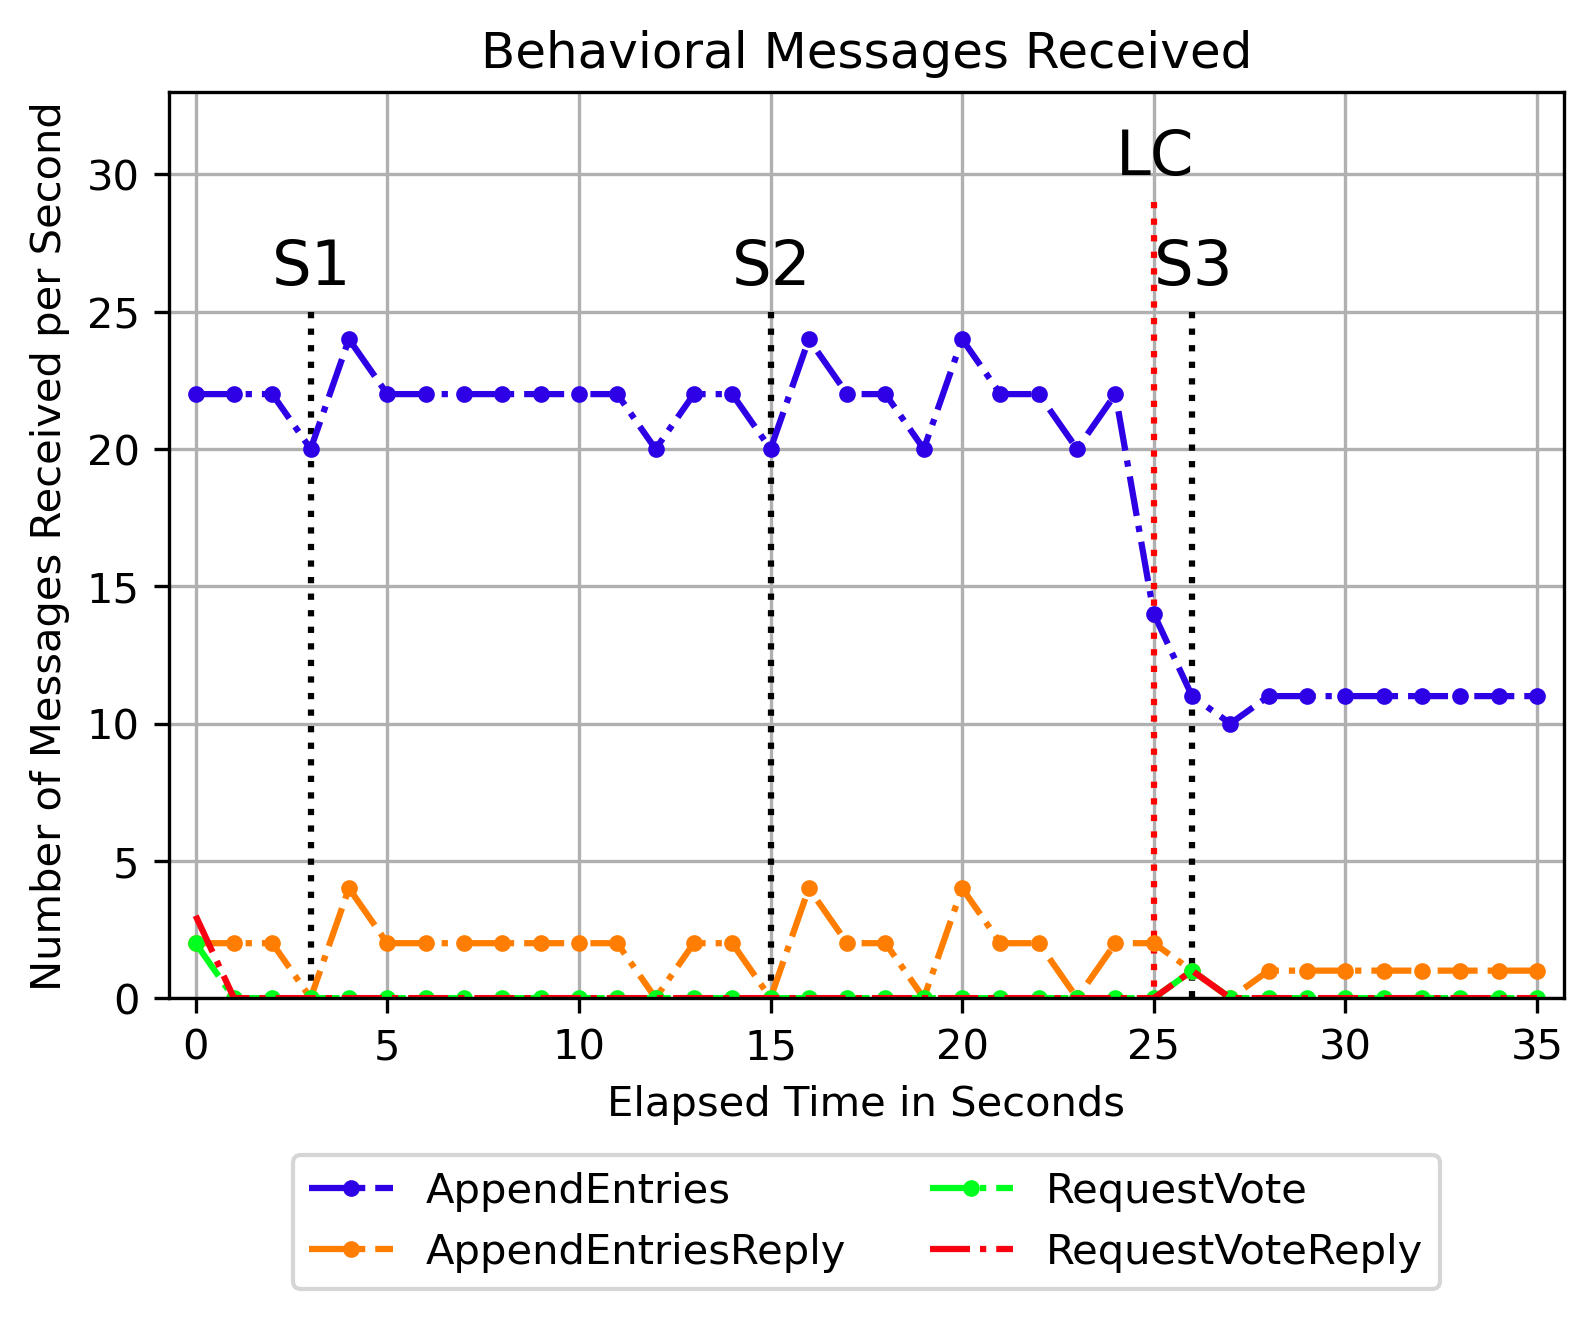
\includegraphics[width=0.8\linewidth]{images/plots/ConsensusMessagesReceive}
	\caption{The number of messages that were received by any replica from behavioral topics throughout three scenarios that start at \textbf{S1}, \textbf{S2}, and \textbf{S3}. After the previous leader crashed at point \textbf{LC}, the number of received messages via the \texttt{AppendEntries} topic decreased by half. This is because heartbeat messages are sent via this topic and the number of followers decreased from two to one after the leader's crash.
}
	\label{fig:PlotConsensusMessagesReceive}
\end{figure}

The effect that a crashed leader - and a crashed replica in general - has on the system is shown in~\autoref{fig:PlotConsensusMessagesReceive}.
After the leader crashed (\textbf{LC}), the number of messages that are received via the \texttt{AppendEntries} topic is reduced by half.
This is due to the fact that only one follower instead of two remains to receive heartbeat messages and requests by the leader.
A difference, on the other hand, can be seen when active hardware redundancy is applied.


\paragraph{Active Hardware Redundancy}

\begin{figure}[!hb]
	\centering
	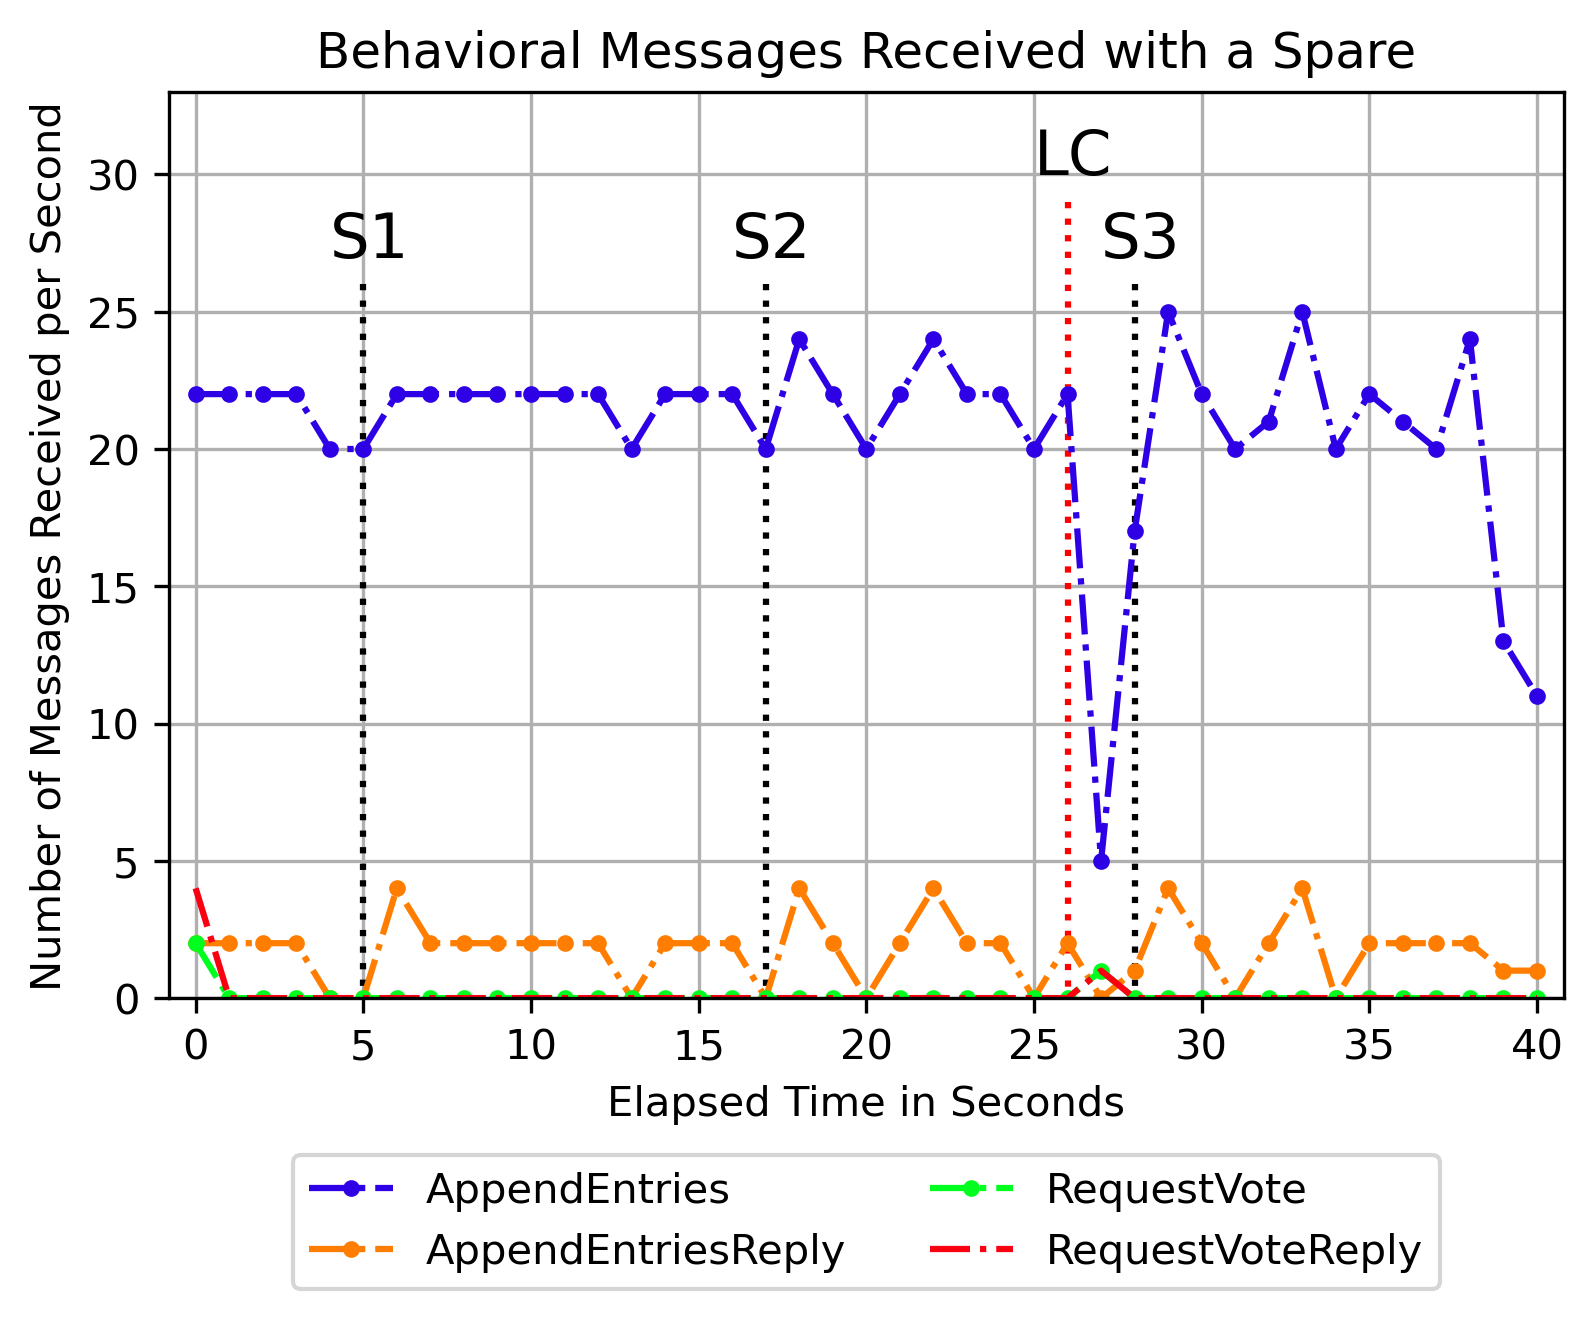
\includegraphics[width=0.8\linewidth]{images/plots/ConsensusMessagesReceiveAHR}
	\caption{The number of messages that were received by any replica from behavioral topics throughout three scenarios that start at \textbf{S1}, \textbf{S2}, and \textbf{S3}. A hot standby was utilized that takes over after the first leader crashed at point \textbf{LC}. After the leader crashed, the number of received messages via the \texttt{AppendEntries} topic dropped. Afterward, a new leader got elected and the spare unit got activated. This is reflected by the fact that the total number of received messages on the \texttt{AppendEntries} topic got back to the amount before \textbf{LC}.}
	\label{fig:PlotConsensusMessagesReceiveAHR}
\end{figure}

In a separate simulation, active hardware redundancy is applied in the form of a hot standby.
Therefore, a fourth replica was added in spare mode.
After the second scenario ended and the third starts, the previous leader was manually stopped (\textbf{LC}).
\\

The total number of messages that are received via behavioral topics is depicted in~\autoref{fig:PlotConsensusMessagesReceiveAHR}.
The crashed leader is evident from the collapse of received heartbeat messages in the system.
Shortly after, a new leader election takes place and the number of received messages on the \texttt{AppendEntries} topic stabilizes.
Unlike in~\autoref{fig:PlotConsensusMessagesReceive}, the number goes back to that before \textbf{LC} showing that there are three active replicas again.


\section{\glsentrylong{DDS}}

\abr{DCPS} systems, such as \abr{DDS}, are designed for machine-to-machine communication in real-time applications~\cite{omgDDSspec}.
\abr{DDS} is designed to facilitate reliable and safe communication in distributes systems.
Therefore, \abr{DDS} was chosen as the basis for the redundant \abr{EVC}.
\\

One challenge of this work, in addition to the suitability of \abr{DDS} for secure and redundant systems, was to find a minimal subset for implementation.
This is because the system, which is designed to function as an \abr{EVC}, requires a \abr{SIL}-level 4~\cite{ChakrabortyFaultTolerantRailway}.
With \abr{DDS} being a significant part in the implementation, the \abr{SIL} of \abr{DDS} needs to be high as well.
With minimal functionality, the cost and time required for approval is also minimal.
\\

At first in this section, the utilized \abr{DDS} subset is described and justified.
Finally, the opportunities and challenges of \abr{DCPS} systems for consensus-based redundant systems are discussed.

\subsection{Subset Selection}

The required subset is determined based on the system requirements.
Secure and reliable communication between different entities should be possible.
Further, communication should be independent of the network topology and the components involved should be able to switch dynamically between being sender and receiver.
In addition to deadlines and time constraints, event-based communication should be enabled.
In this way, the \abrpl{RPC} proposed by \texttt{Raft} can be emulated.
Additionally, a global system state should be managed by \abr{DDS}.
\\

The \abr{DCPS} part of \abr{DDS} is divided into five modules that each fulfills a different task.
Throughout this section, the used subset for each of the five modules is described.
\\

The overview of used functionality only contains methods that are directly used by the application.
However, the middleware might transitively utilize additional functionalities to implement the features mentioned in this system.

\paragraph{Domain Module}
A \abr{DDS} application's main building blocks comprise a \texttt{Domain}, one or multiple \texttt{DomainParticipants}, as well as a \texttt{DomainParticipantFactory} for creating new \texttt{DomainParticipants}~\cite{omgDDSspec}.
Besides these classes, the domain module contains various functionalities, from which the following subset is used within the exemplary implementation.

\begin{itemize}
\item \textit{DDS\_DomainParticipant\_create\_(publisher|subscriber|topic)} Is used for creating \abr{DDS} publishers, subscribers or topics.
\item \textit{DDS\_DomainParticipant\_delete\_(publisher|subscriber|topic)} Is used for deleting \abr{DDS} publishers, subscribers or topics.
\item \textit{DDS\_DomainParticipantFactory\_get\_instance} Used for acquiring the \texttt{DomainParticipantFactory} singleton.
\item \textit{DDS\_DomainParticipantFactory\_(create|delete)\_participant} Used for creating and deleting a new participant in the \abr{DDS} domain.
\end{itemize}


\paragraph{Publication Module}
\texttt{Publishers}, as well as \texttt{DataWriters}, which are used for data distribution, are located within the publication module.
Besides these two classes, the following functionality is required for the exemplary implementation:

\begin{itemize}
\item \textit{DDS\_Publisher\_(create|delete)\_datawriter} Used for creating, respectively deleting, \texttt{DataWriter} objects.
\item \textit{DDS\_DataWriter\_write} Used for writing new data to an instance on a \abr{DDS} topic.
\item \textit{DDS\_DataWriter\_dispose} Used for marking processed inputs for deletion so that they are not processed twice and for disposing outdated state instances.
\item \textit{DDS\_DataWriter\_(register|unregister)\_instance} Used for locking and unlocking instance resources from the middleware before reading or modifying them. For example used for the linked balises in the global state.
\item \textit{DDS\_DataWriter\_lookup\_instance} Used for getting the corresponding instance before disposing it.
\end{itemize}


\paragraph{Subscription Module}
The subscription module resembles the publication module but for reading and receiving data.
However, besides \texttt{Subscribers} and \texttt{DataReaders}, it also contains \texttt{DataSample}, \texttt{SampleInfo}, and \texttt{ReadCondition}.
\texttt{Subscribers} and \texttt{DataReaders} are required for receiving data, which is represented by a \texttt{DataSample}.
The \texttt{SampleInfo} data structure contains additional information for each \texttt{DataSample}, such as its instance handle or state, which makes it mandatory for the implementation as well.
\texttt{ReadConditions} are used in combination with \texttt{WaitSets}, so that the application can react to certain middleware states.

Further, the following functionalities from the subscription module were used:

\begin{itemize}
\item \textit{DDS\_Subscriber\_(create|delete)\_datareader} Used for creating, respectively deleting, \texttt{DataReaders}.
\item \textit{DDS\_DataReader\_(create|delete)\_readcondition} Used for creating, respectively deleting, \texttt{ReadConditions}.
\item \textit{DDS\_DataReader\_read} Used to read data from a \texttt{DataReader} but not removing it. This is required for input messages that are only allowed to be removed when they are entirely processed and for state data.
\item \textit{DDS\_DataReader\_take} Used for reading and removing data from a \texttt{DataReader}.
\item \textit{DDS\_DataReader\_return\_loan} Required for indicating the middleware that the application finished accessing a sequence of data. This allows the middleware to work with the data again.
\end{itemize}

\paragraph{Topic-Definition Module}
The topic definition module contains everything related to topics.
The exemplary implementation utilizes \texttt{Topics}, for describing data in the application, and \texttt{TypeSupport} which describes a data type bound to a \texttt{Topic}.
Apart from these two classes, the following methods are used:

\begin{itemize}
\item \textit{DDS\_TypeSupport\_\_alloc} Used for creating a new \texttt{TypeSupport}.
\item \textit{DDS\_TypeSupport\_get\_type\_name} Used for getting a data type's default name required to register it later on.
\item \textit{DDS\_TypeSupport\_register\_type} Used for registering a new data type name on a \texttt{DomainParticipant}.
\end{itemize}

\paragraph{Infrastructure Module}
The classes that are used from the infrastructure module include \texttt{QosPolicy} and \texttt{WaitSet}.
The \texttt{QosPolicy} class implements \abr{DDS}'s \abr{QOS} functionalities and is therefore mandatory for the system's correctness.
\texttt{WaitSets} are applied for ensuring the application's compliance with its time restrictions because they allow the assignment of timeouts.
In addition to that, the following functionalities from the infrastructure module are applied:

\begin{itemize}
\item \textit{DDS\_WaitSet\_\_alloc} Used for creating new \texttt{WaitSets}.
\item \textit{DDS\_WaitSet\_(attach|detach)\_condition} Used to attach and detach a condition to the corresponding \texttt{WaitSet}.
\item \textit{DDS\_WaitSet\_wait} Stops the according thread until at least one of the attached conditions evaluates to true.
\end{itemize}

\paragraph{Quality of Services}
The \texttt{QosPolicy} class is part of the infrastructure module.
It allows defining \abr{QOS} policies that regulate how the middleware transmits and stores data.
The following \abr{QOS} policies are used in the application:

\begin{itemize}
\item DDS\_DestinationOrderQosPolicy: Controls the order in which \texttt{DataReaders} store the data.
	\begin{itemize}
	\item DDS\_BY\_SOURCE\_TIMESTAMP\_DESTINATIONORDER\_QOS: Used for every topic.
	\end{itemize}
\item DDS\_DurabilityQosPolicy: Controls whether the data should be stored for late joining readers.
	\begin{itemize}
	\item DDS\_VOLATILE\_DURABILITY\_QOS: The system by design ensures that a sufficient number of replicas is active. Late joining replicas do not need to react to previous events.
	\item DDS\_PERSISTENT\_DURABILITY\_QOS: Used for the enduring state topic so that late joining replicas can make decisions based on recent global state and input topic so that no input is lost.
	\end{itemize}
\item DDS\_HistoryQosPolicy: Controls how many revisions of a sample are stored.
	\begin{itemize}
	\item DDS\_KEEP\_ALL\_HISTORY\_QOS: Used so that all events are eventually processed and none is lost.
	\item DDS\_KEEP\_LAST\_HISTORY\_QOS: For state topics, only the most recent sample is important.
	\end{itemize}
\item DDS\_LifespanQosPolicy: Specifies how long data samples are valid. For example, the decision-making process has time restrictions, so that decision requests expire.
\item DDS\_ReliabilityQosPolicy: Controls the communication's reliability.
	\begin{itemize}
	\item DDS\_RELIABLE\_RELIABILITY\_QOS: Used to ensure that no events are lost and that each replica has the most recent global state.
	\item DDS\_BEST\_EFFORT\_RELIABILITY\_QOS: The \texttt{TrainState} topic, being a volatile state, does not necessarily require reliable communication.
	\end{itemize}
\item DDS\_ResourceLimitsQosPolicy: Controls the maximum amount of resources used by \texttt{DataReaders} and \texttt{DataWriters}. Required because the application is supposed to run in a resource-constrained environment.
\end{itemize}


The \abr{ETCS} subset studied in this paper serves as a model for \abr{ETCS} in general.
Therefore, the elaborated \abr{DDS} subset is pertinent for the overall \abr{ETCS} specification.
However, for a \abr{SIL} 4 system, the \abr{SIL} level of the applied \abr{DDS} application must be sufficient. Furthermore, for a \abr{SIL} 4-compliant system, the used components must also fulfill a certain \abr{SIL} level.
The required component \abr{SIL}-level as well as the \abr{DDS} application's SIL-level are left to future work.

\subsection{Opportunities and Challenges}

In this section, the suitability of \abr{DCPS} systems, like \abr{DDS}, for consensus-based redundant systems is discussed.

\paragraph{Advantages}
On the one hand, \abr{DDS} allows to utilize \abr{QOS} settings to specify what is expected from the system rather than how it should be done.
Through \texttt{ReadConditions}, messages can be filtered.
Further, \texttt{WaitSets} and \abr{QOS}-settings can be used to declare time restriction and requirements.
This facilitates reliable and predictable machine-to-machine communication.

In addition, the middleware supports the automatic discovery of replicas to that the number of used replicas is dynamically scalable.
For example, an active spare unit can be added to the system at any time and is automatically discovered and included.
This would also allow to apply a three-out-of-five system rather than a two-out-of-three system and use the same software.

Finally, \abr{DDS} supports fast transmission times and manageable hardware utilization, as shown in measurements.
All in all, the functionalities of DDS simplify secure and time-critical communication, as well as procedures.

\paragraph{Challenges}
On the other hand, the \abr{DDS} standard has been designed around a loose coupling of publishing and subscribing components.
However, decoupling of senders and receivers is not always possible in a consensus-based and safety-critical redundant system.
A follower replica that receives heartbeat messages can become the sender of heartbeat messages at any time when the previous leader becomes unavailable.
Therefore, replicas need to alternate dynamically between sending and receiving data.
One way to solve this challenge is to create and delete objects for publishing and subscribing to topics dynamically.
However, this can lead to a sudden allocation and deallocation of dynamic memory, leading to unpredictable timings.
Thus, every replica allocates the required objects to publish and subscribe to every topic at program start, which leads to other challenges.
\\

When each replica is subscribed to a topic that applies a \texttt{History}- and \texttt{ResourceLimit} \abr{QOS}, the messages that are received by \texttt{DataReader} objects must be taken by the application.
Hence, a leader that is subscribed to the \texttt{AppendEntries} topic in preparation of becoming a follower must take all heartbeat messages from the topic published by itself.
This introduces a computational overhead, though a small one as the system's resource utilization in~\autoref{fig:PlotCPUUsageIdleTime} show.
\\

Lastly, a system that utilizes \abr{DDS} for communication needs to support concurrent computations when more than one message should be processable at any time.
This introduces potential race conditions or deadlocks and can complicate the development and approval process.
Since the developed system, for example, needs to react to vote requests and log replication messages at any time, a concurrent system design is unavoidable.
However, as described in~\autoref{subsub:raceConditions}, the implemented concurrent algorithm keeps the probability of race conditions small.
All in all, the use of \abr{DDS} can increase the development effort on the one hand. However, on the other hand, it offers functionalities to simplify and ensure the security and implementation of time-critical applications.



\iffalse


\todo{Integrate the following into the text}
For every message that is published or received by a replica, an entry is written into another file.
Thereby, not only the system's final decision, but also the replica's synchronization to come to an agreement can be understood.

\paragraph{Send Messages Size}
\begin{figure}[!htb]
	\centering
	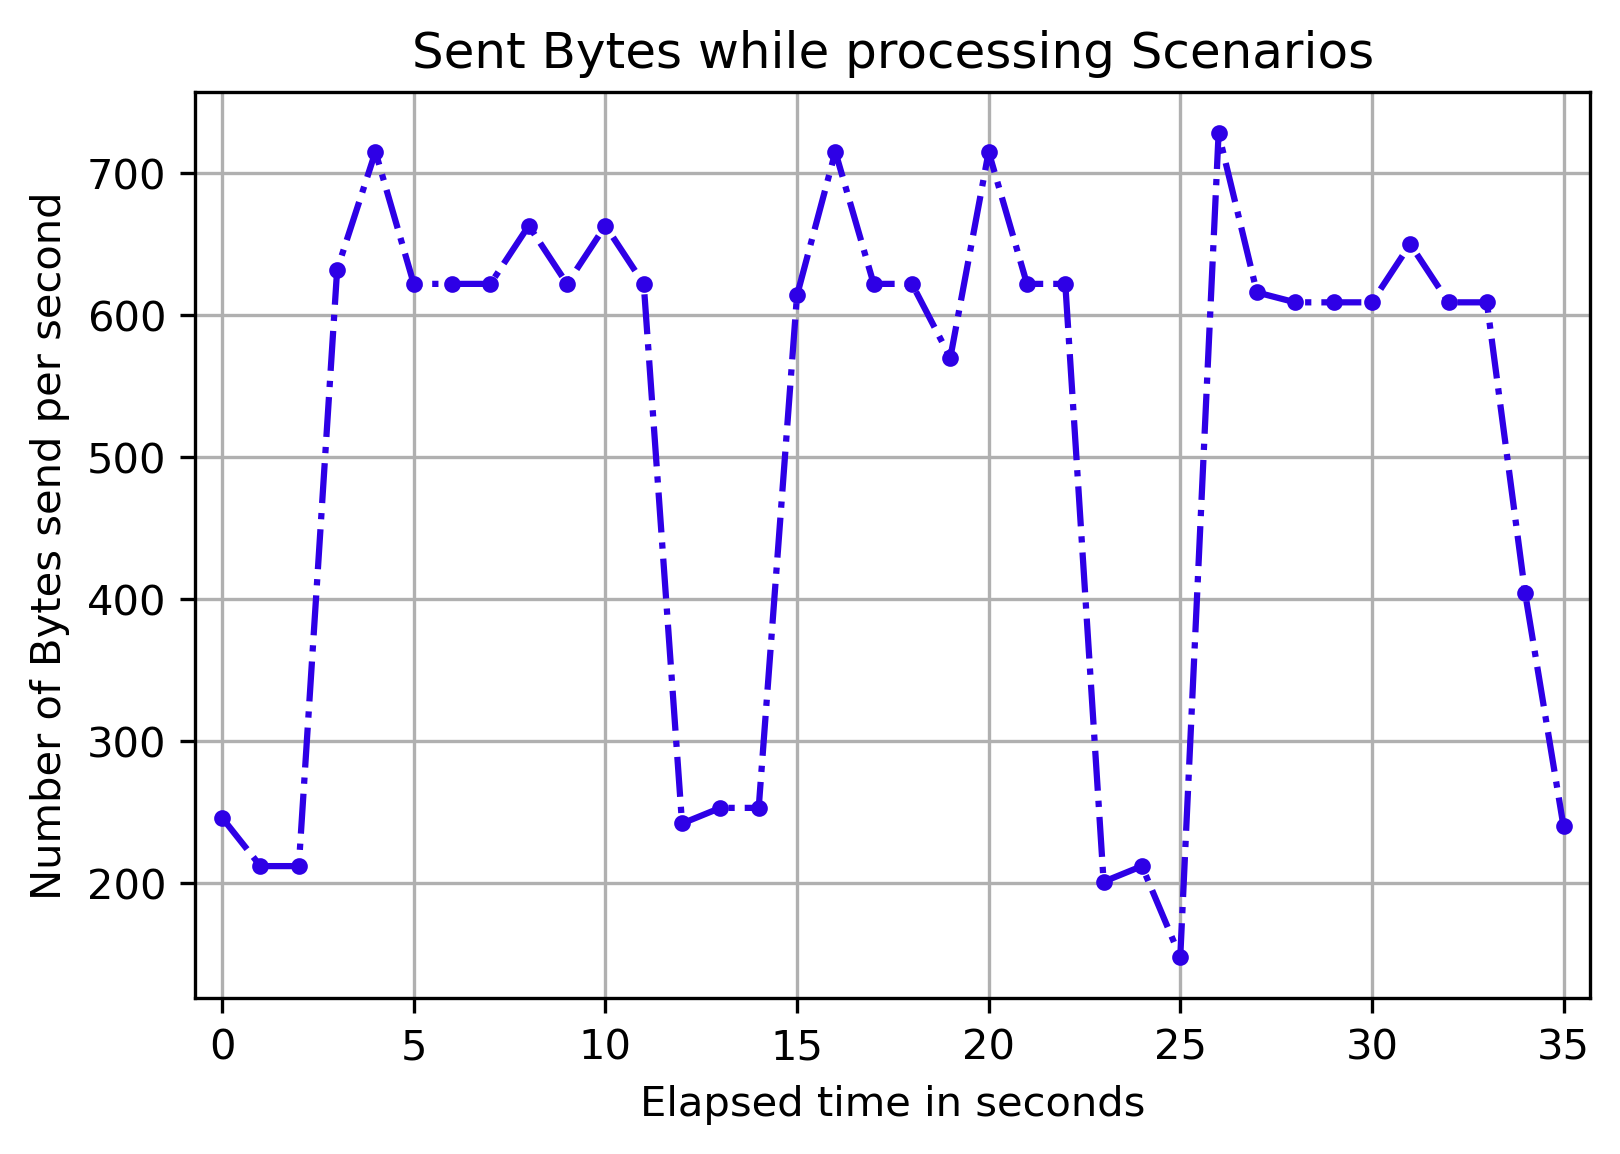
\includegraphics[width=0.75\linewidth]{images/plots/scenarioProcessingMessageSize}
	\caption{TODO}
	\label{fig:messageSizeScenarioProcessing}
\end{figure}


\paragraph{Total Messages Received}

\begin{figure}[!htb]
	\centering
	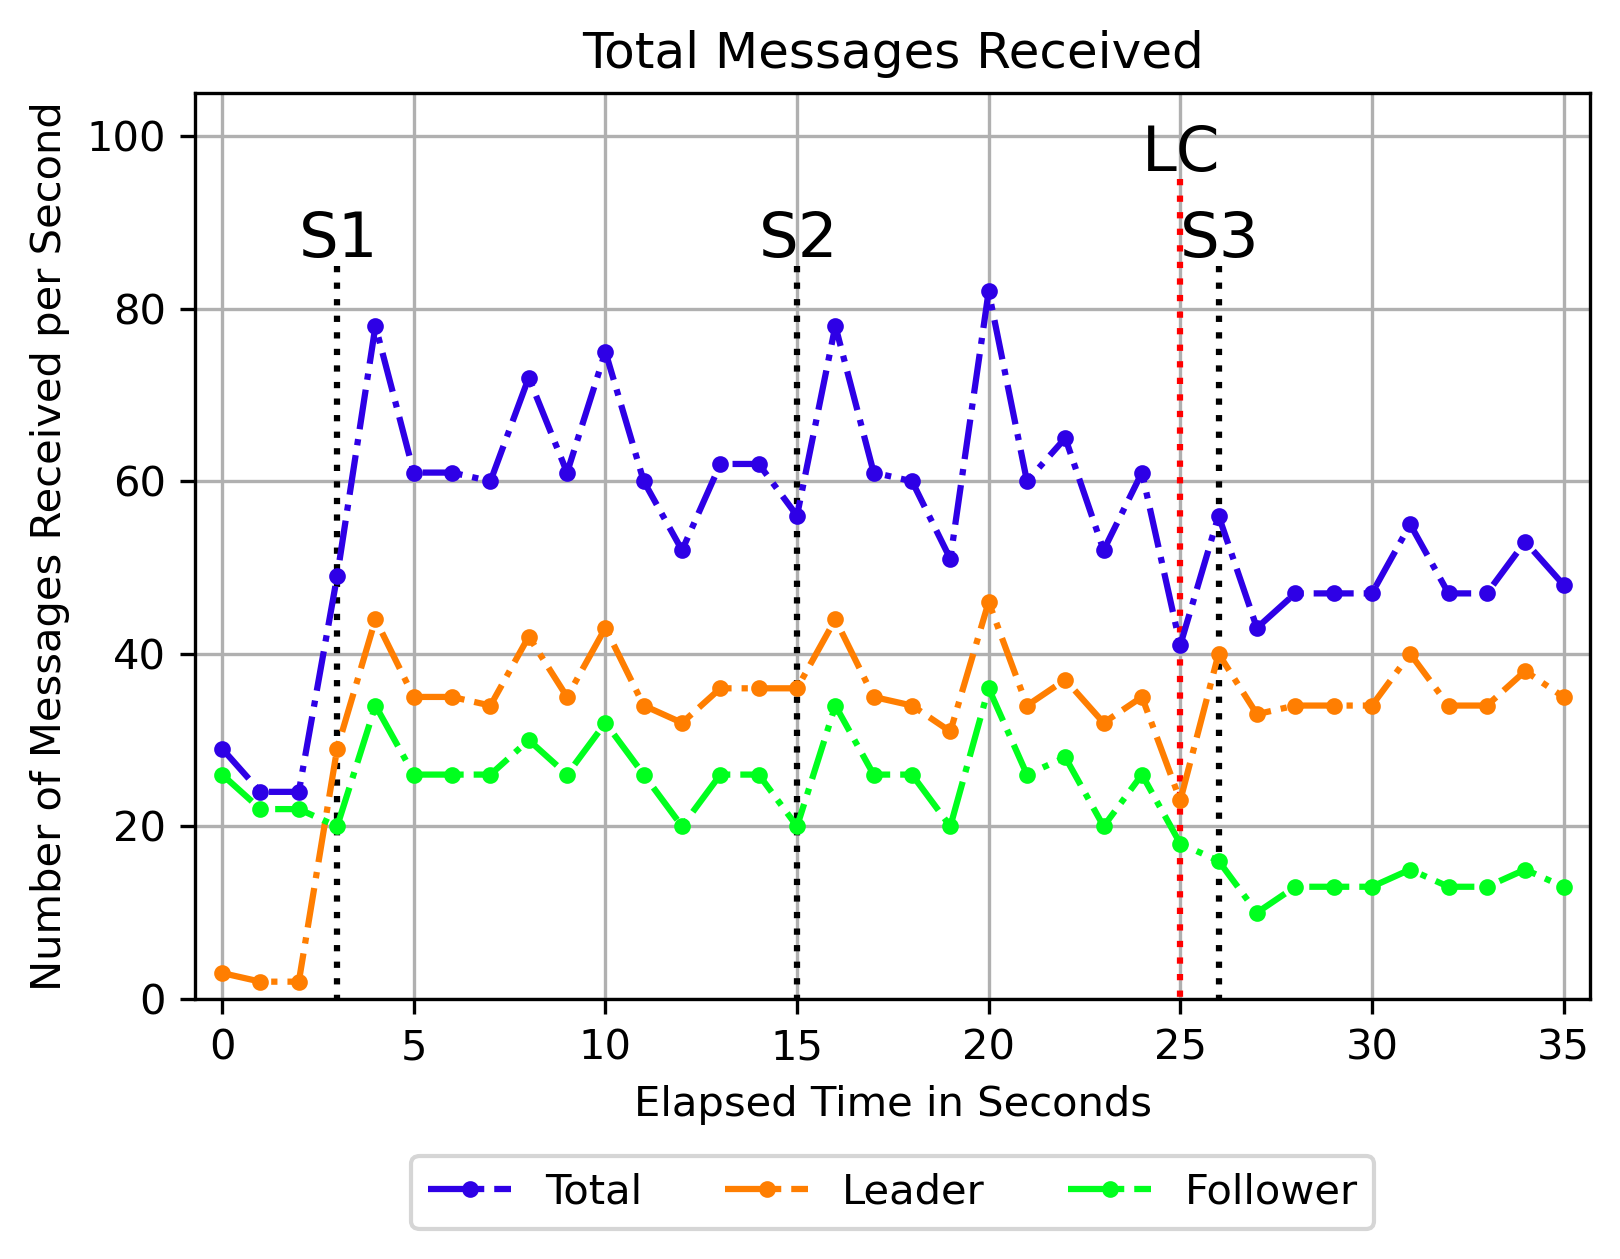
\includegraphics[width=0.75\linewidth]{images/plots/TotalMessagesReceive}
	\caption{Overview about all messages that are received from replicas within the system.}
	\label{fig:PlotTotalMessagesReceive}
\end{figure}

The total number of messages received through \abr{DDS} topics can be seen in~\autoref{fig:PlotTotalMessagesReceive}.
What is interesting is, that the leader receives and reads more messages than the two followers combined.
This is mostly because the leader is responsible for reading the input topic and because it receives and reads messages from both followers.
Another interesting circumstance can be seen after 25 seconds - which is when the previous leader crashes - since the amount of messages that the followers received is halved.
This is because only one, instead of two, followers remain in the system.



\begin{table}[h!]
	\begin{center}
		\caption{All topics that are utilized in the system have a certain data schema. From the resulting message size, the transmission time in the system can be calculated. The size and transmission time of the \texttt{AppendEntries} and \texttt{Input} depends on the length of the data sequence (\textbf{l}).}
		\label{tab:topicSendingTimes}
		\begin{tabularx}{\textwidth}{|X|X|}
			\hline
			\textbf{Topic} & \textbf{Message Size in Bytes} \\
			\hline \hline
			AppendEntries & $12 + 4 * l$ & $0.402768 * l + 3219.11$ \\
			\hline
			AppendEntriesReply & 18 & 3219.7 \\
			\hline
			RequestVote & 8 & 3218.7 \\
			\hline
			RequestVoteReply & 13 & 3219.21 \\
			\hline
			Input & $4 + 4 * l$ & $0.402768 * l + 3218.3$ \\
			\hline
			ActivateSpare & 5 & 3218.40 \\
			\hline
			LinkedBalises & 6 & 3218.5 \\
			\hline
			TrainState & 41 & 3222 \\
			\hline
			MovementAuthority & 8 & 3218.7 \\
			\hline
		\end{tabularx}
	\end{center}
\end{table}


\paragraph{Data Transmission Time}
\begin{figure}[!htb]
	\centering
	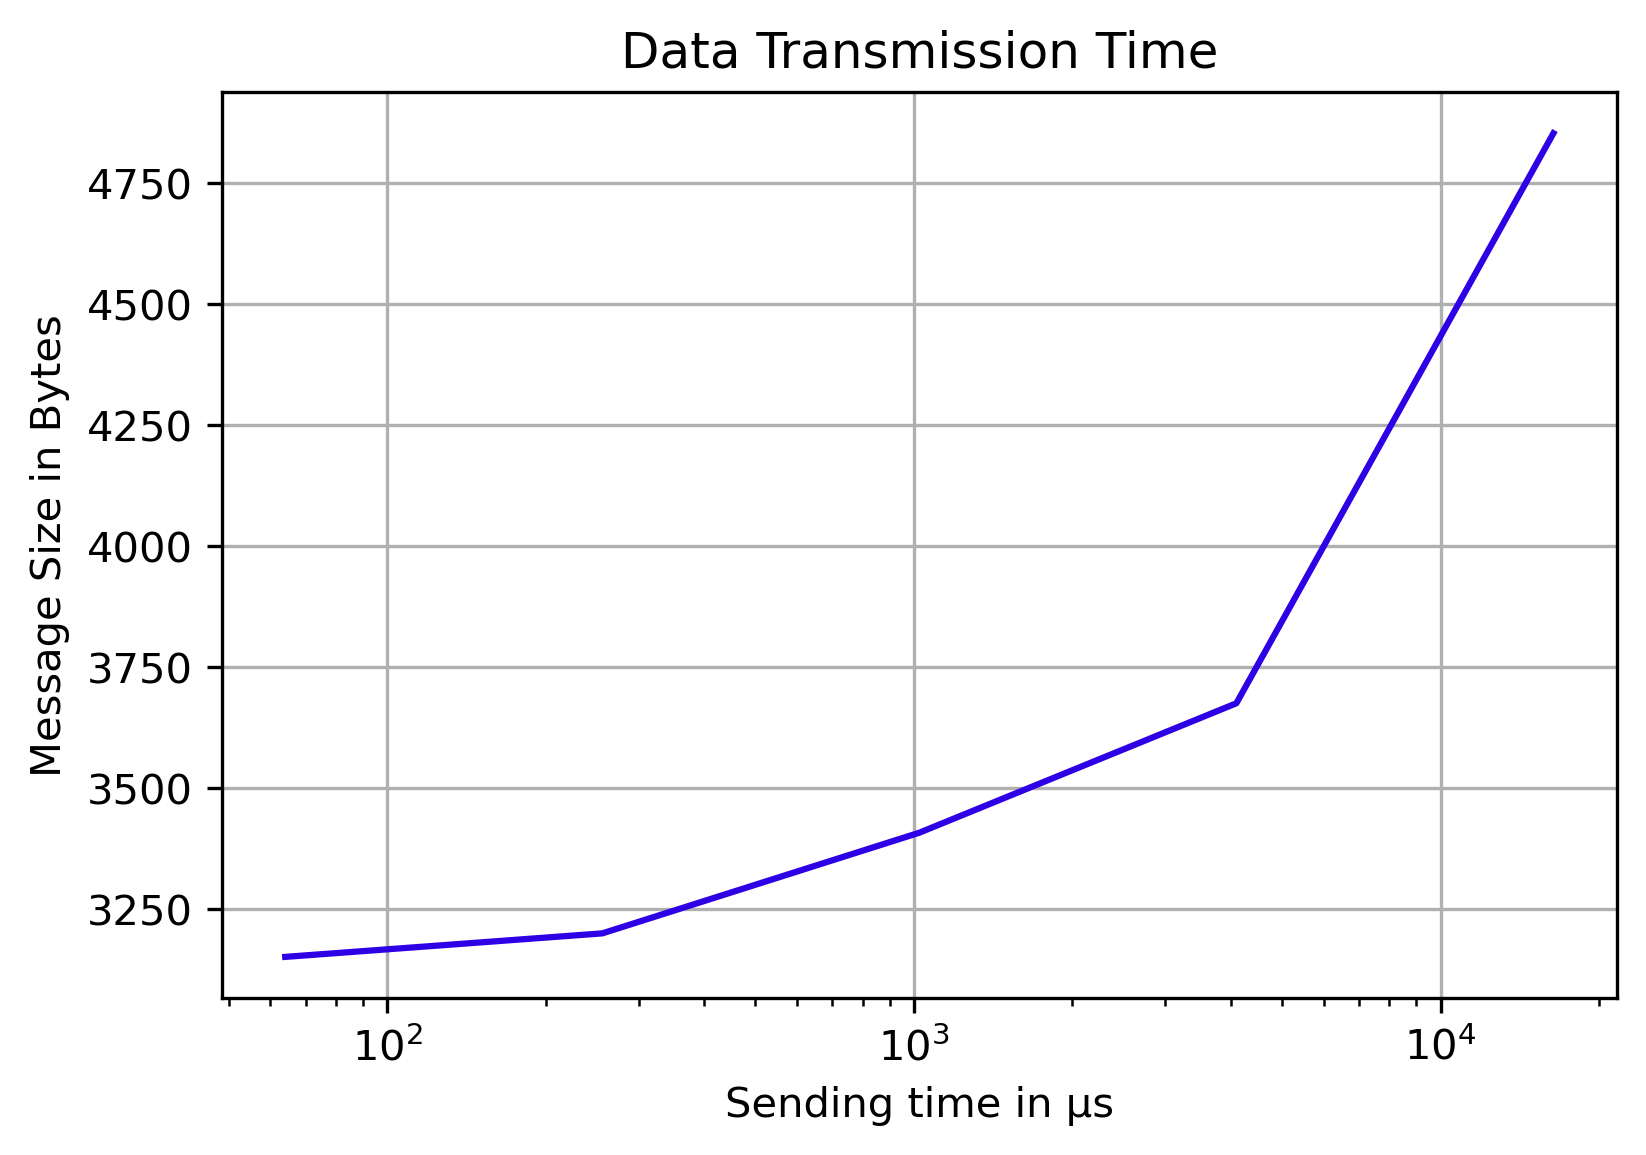
\includegraphics[width=0.75\linewidth]{images/plots/sendingTimes}
	\caption{Time that is required to transmit messages with different payload sizes via a \abr{DDS} topic. The times were determined by calculating the mean sending time out of 200 messages per payload size.}
	\label{fig:PlotSendingTimes}
\end{figure}


Further, the time that is required to publish and process a message with a certain payload size between two replicas via a \abr{DDS} topic is measured.
For bypassing clock skews in the system, a request/response approach is used, where one replica publishes a message with a certain payload size and waits until another replica confirms the message's receipt.
The receiving replica constantly checks for new messages and, as soon as it receives one, publishes a confirmation messages on another topic.
Any time that is required to send the confirmation message is negligible because it only consists of a 8-bit identification number that assigns it to a payload carrying message.
The results, which are shown in~\autoref{fig:PlotSendingTimes}, were determined by measuring the time that elapsed between sending a message and receiving the corresponding confirmation.
This process was repeated 200 times for each payload size and a mean was calculated.
What emerged is, that the transmission time is directly dependent on the published message's size.



\paragraph{State Messages Received}

\begin{figure}[!htb]
	\centering
	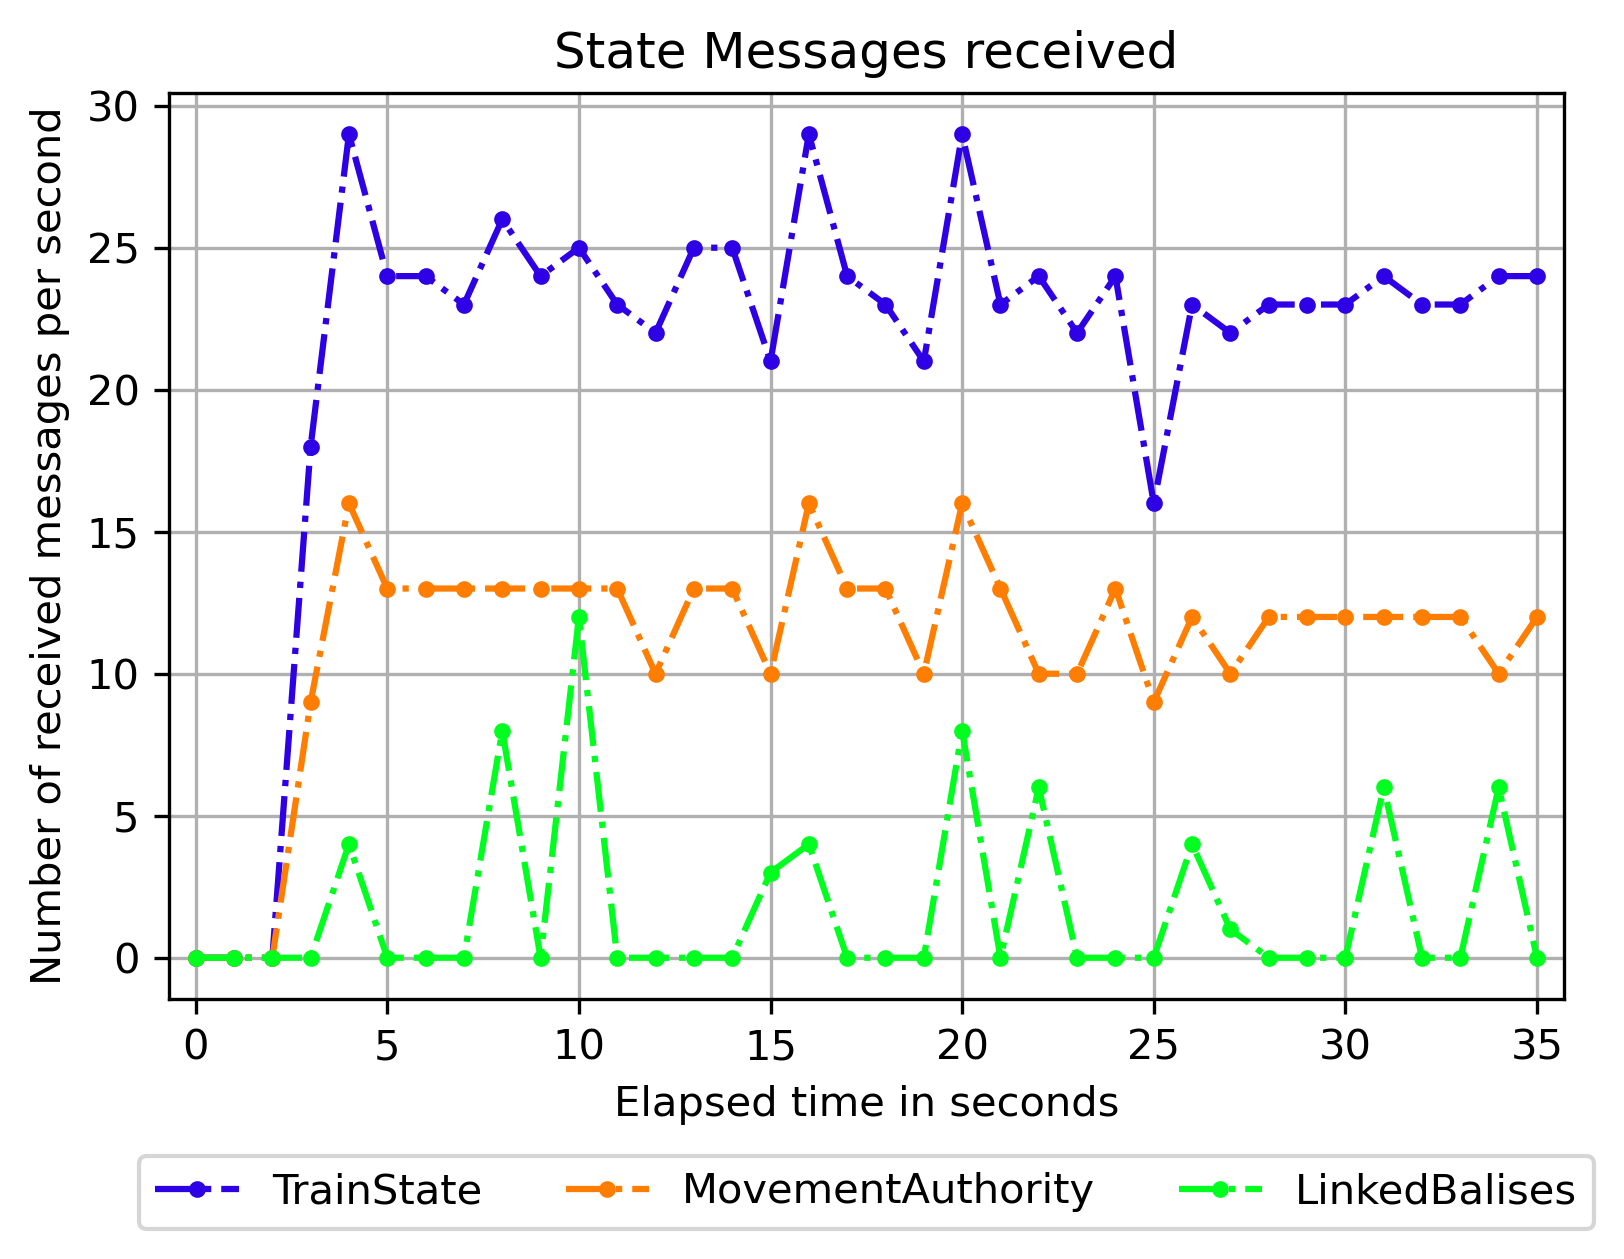
\includegraphics[width=0.75\linewidth]{images/plots/StateMessagesReceive}
	\caption{}
	\label{fig:PlotStateMessagesReceive}
\end{figure}


Do experiement and structure in way such as SakicTimeInConsensus

Leader stable for 45 minutes with 500000x07x2

For the tranmit time, I measured 20 messages each time and took the average (calculate standard deviation)
\fi
